\documentclass[a4paper,12pt, oneside]{book}

%\usepackage{fullpage}
\usepackage[T1]{fontenc}
\usepackage[italian]{babel}
\usepackage[utf8]{inputenc}
\usepackage{amssymb}
\usepackage{amsthm}
\usepackage{mathtools}
\usepackage{graphics}
\usepackage{amsfonts}
\usepackage{listings}
\usepackage{amsmath}
\usepackage{amstext}
\usepackage{engrec}
\usepackage{rotating}
\usepackage[safe,extra]{tipa}
\usepackage{showkeys}
\usepackage{multirow}
\usepackage{hyperref}
\usepackage{microtype}
\usepackage{enumerate}
\usepackage{braket}
\usepackage{marginnote}
\usepackage{pgfplots}
\usepackage{cancel}
\usepackage{polynom}
\usepackage{booktabs}
\usepackage{enumitem}
\usepackage{framed}
\usepackage{pdfpages}
\usepackage{pgfplots}
\usepackage[usenames,dvipsnames]{pstricks}
\usepackage{epsfig}
\usepackage{pst-grad} % For gradients
\usepackage{pst-plot} % For axes
\usepackage[space]{grffile} % For spaces in paths
\usepackage{etoolbox} % For spaces in paths
\makeatletter % For spaces in paths
\patchcmd\Gread@eps{\@inputcheck#1 }{\@inputcheck"#1"\relax}{}{}
\makeatother
\usepackage[cache=false]{minted}
\usepackage{fancyhdr}
\newcommand{\numberset}{\mathbb}
\newcommand{\N}{\numberset{N}}
\newcommand{\Z}{\numberset{Z}}
\newcommand{\Q}{\numberset{Q}}
\newcommand{\R}{\numberset{R}}

\pagestyle{fancy}
\fancyhead[LE,RO]{\slshape \rightmark}
\fancyhead[LO,RE]{\slshape \leftmark}
\fancyfoot[C]{\thepage}



\title{Probabilità e Statistica per l'Informatica}
\author{UniShare\\\\Davide Cozzi\\\href{https://t.me/dlcgold}{@dlcgold}\\\\Gabriele De Rosa\\\href{https://t.me/derogab}{@derogab} \\\\Federica Di Lauro\\\href{https://t.me/f_dila}{@f\textunderscore dila}}
\date{}

\pgfplotsset{compat=1.13}
\begin{document}
\maketitle
\tableofcontents

\definecolor{shadecolor}{gray}{0.80}

\newtheorem{teorema}{Teorema}
\newtheorem{definizione}{Definizione}
\newtheorem{esempio}{Esempio}
\newtheorem{corollario}{Corollario}
\newtheorem{lemma}{Lemma}
\newtheorem{osservazione}{Osservazione}
\newtheorem{nota}{Nota}
\newtheorem{esercizio}{Esercizio}
\newcommand{\mean}[1]{\overline #1}
\renewcommand{\chaptermark}[1]{%
\markboth{\chaptername
\ \thechapter.\ #1}{}}
\renewcommand{\sectionmark}[1]{\markright{\thesection.\ #1}}
\chapter{Introduzione}
\textbf{Questi appunti sono presi a lezione. Per quanto sia stata fatta una revisione è altamente probabile (praticamente certo) che possano contenere errori, sia di stampa che di vero e proprio contenuto. Per eventuali proposte di correzione effettuare una pull request. Link: } \url{https://github.com/dlcgold/Appunti}.\\
\textbf{Grazie mille e buono studio!}

La statistica è una discliplina, basata sulla matematica, con finalità lo studio quantitativo e qualitativo
di un particolare fenomeno collettivo, in condizioni di incertezza o non determinismo ed è usata in molti 
ambiti, come ad esempio l'intelligenza artificiale, data science, robotica, domotica e tutte le analisi 
per poter ottenere ricavare delle informazioni sui dati.

Si ha l'\emph{A-B testing}, per decidere tra due scelte la migliore e per la decisione si analizzano i dati
presi da campioni di popolazione, utilizzando il \emph{tasso di conversione}, ossia la percentuale di visitatori unici
che hanno effettuato la azione su cui si sta effettuando il test.

In questo corso verranno affrontati e studiati i seguenti argomenti:
\begin{enumerate}
    \item statistica descrittiva
    \item calcolo delle probabilità
    \item distribuzioni notevoli
    \item teoremi di convergenza
    \item stima dei parametri
    \item test di ipotesi parametrici
    \item test di ipotesi non parametrici
    \item regressione lineare
\end{enumerate}

\chapter{Statistica Descrittiva}
La statistica descrittiva è una raccolta di metodi e strumenti matematici usati per organizzare una o più serie di dati
al fine di trovarne delle simmetrie, periodicità o delle eventuali leggi.

Solitamente i dati disponibili non rappresentano tutta la popolazione ma un numero limitato 
di osservazioni effettuato su un \emph{campione}, sottoinsieme selezionato della popolazione su cui si effettua
l'analisi statistica, la cui efficacia dipende da quale sottoinsieme è stato scelto, infatti non esiste 
un solo campione ma vi sono diversi modi per sceglierli, più o meno efficaci, per l'analisi statistica.

Quando si effettua un analisi statistica si vuole affermare qualcosa riguardo i \emph{caratteri} della popolazione,
ossia gli elementi su cui si effettua l'analisi statistica, che possono essere:
\begin{itemize}
    \item \emph{caratteri qualitativi}, indicanti qualità (colori, stili, materiali etc...) e anche dati non numerici
             in cui solitamente non è definita una \textit{relazione d'ordine}
    \item \emph{caratteri quantitativi}, maggiormente studiati dal corso, dati numerici 
          in cui vengono definite \emph{relazioni d'ordine}, che possono essere a loro volta divisi in
          \emph{discreti}, indicanti valori in $\Z$, e \emph{continui}, con valori nel campo $\R$.
\end{itemize}
Supponiamo di considerare $n$ elementi della popolazione e di rilevare, per ognuno di essi,
il dato relativo al carattere quantitativo da esaminare, ossia definiamo l'insieme di dati
$E=\{x_1, x_2, \dots, x_n\}$ con la numerosità, il numero di elementi considerati, pari a $n$.

In caso il carattere è discreto è comodo raggruppare i dati considerando l'insieme di tutti i valori assumibili,
detta \emph{modalità del carattere} ed associare ad ognuno di esso il numero di volte che esso compare in $E$.\newline
Si ha quindi il numero di totalità $N$ del carattere e si definisce l'insieme di modalita $S=\{s_1,...,s_N\}$
su cui si definiscono i seguenti valori statistici:
\begin{description}
    \item [frequenza assoluta ] numero di volte $f_j$ che si ha un elemento di un campione
    \item [frequenza cumulata assoluta] somma delle frequenze assolute di tutte le modalità, 
           indicato con $F_j$, calcolato con la seguente formula:
            \[ F_j = \sum_{k:s_k \leq s_j} f_k \]
    \item [frequenza relativa] rapporto tra la frequenza assoluta e il numero di elementi,
           indicata con $p_j$, calcolata come 
            \[ p_j = \frac{f_j}{n} \]
    \item [frequenza cumulativa relativa $P_j$] somma delle frequenze relativa di tutte le modalità,
           indicato con $P_j$, calcolata come 
            \[ P_j = \sum_{k:s_k \leq s_j} p_k \]
\end{description}
Si definisce \emph{distribuzione di frequenza} una funzione $F:S \to \N$ che associa ad ogni modalità 
la corrispondente frequenza, per cui esiste la distribuzione di frequenza assoluta, relativa, 
frequenza cumulativa assoluta e relativa.

%inserire esempio pagina 9
Quando il carattere da studiare è continuo o discreto con un gran numero di valori, è conveniente 
ricondursi a raggruppamenti come quelli appena trattati, per cui si suddivide l'insieme delle modalità $S$,
in alcune classi, sottoinsiemi di $S$, che formano una partizione.\newline
La scelta delle classi con cui si suddivide l'insieme $S$ è del tutto arbitraria anche se è necessario
che esse formino una partizione di $S$.\newline
Le partizioni devono essere significative e sufficientemente numerose ed inoltre ad ogni classe si associano le grandezze:
confini superiori ed inferiori, l'ampiezza e il valore centrale della classe.

Nel caso in cui il carattere esaminato sia continuo occorre specificare come le classi sono chiuse, a destra o a sinistra,
ossia specificare se gli elementi dell'indagine il cui dato coincide con il confine della classe sono da raggruppare
all'interno della classe stessa oppure no.
%esempio a pagina 13
\section{Indici di tendenza Generale}
Fino ad ora abbiamo visto come rappresentare i dati, ora iniziamo ad analizzare gli indici
che ci forniscono un valore che rappresenta un certo aspetto della serie di dati, 
incominciando dagli \emph{indici di tendenza generale}:
\begin{description}
    \item [media] è la media aritmetica tra tutti i valori dei dati osservati 
            \[ \overline{x} = \frac{1}{n} \sum x_i = \frac{x_1 + \cdots + x_n}{n} \]
            Considerando le distribuzioni di frequenza definite, posssiamo fornire definizioni equivalenti di media:
                \[ \overline{x} = \frac{1}{n} \sum s_j f_j = \sum s_j p_j \]
                La dimostrazione dell'uguaglianza di queste definizioni alternative è banale e si riconduce 
                alla definizione di frequenza relativa ed assoluta.

    \item [mediana] è l'elemento in mezzo ai valori dei dati, ordinati in maniera crescente
            in cui se il numero degli elementi $n$ è dispari è l'elemento $\frac{n + 1}{2}$
            altrimenti è la somma degli elementi di posto $\frac{n}{2}$ e $\frac{n}{2} + 1$.

    \item [moda] valore o classe, indicato con $\widetilde{x}$, corrispondente alla massima frequenza assoluta
                 e viene usata solitamente in caso sia impossibile definire la media e la mediana.\newline
            La moda non è unica infatti parliamo di \emph{distribuzione uni-modale}, nel caso di un'unica moda,
            altrimenti di \emph{distribuzione multi-modale}.
\end{description}
%aggiungo esempio
Gli indici di tendenza centrale non sono utili per fornire informazioni circa l'omogeneità dei dati, in quanto forniscono 
informazioni sui valori centrali e medi del campione statistico, per cui per risolvere sto problema
introduciamo i seguenti indici:
\begin{description}
        \item [varianza] è la media dello scarto quadratico di ogni elemento dalla sua media 
                \[ s^2 = \frac{1}{n} \sum _{i = 1} ^ n (x_i - \overline{x})^2 \]
                La varianza ovviamente è tanto più grande quanto i singoli elementi si discostano dalla media, 
                ossia significa che i dati in tal caso sono molto disomogenei.\newline
                Come abbiamo già visto per la media sono presenti le seguenti definizioni alternative di varianza:
                \[ s^2 = \frac{1}{n} \sum _{j = 1} ^ N f_j (s_j - \overline{x}) ^ 2 \]
                \[ s^2 = \sum _{j = 1} ^ N p_j (s_j - \overline{x}) ^ 2 \]
                \[ s^2 = \sum _{j = 1} ^ n x_j - \overline{x} ^ 2 \]
                Le prime due definizioni alternative derivano dalla definizione di frequenza assoluta e frequenza 
                mentre l'ultima proviene da passaggi algebrici, dimostrati di seguito formalmente:
                \begin{proof}
                        \[ \begin{split}
                            s^2 & = \frac{1}{n} \sum _{i = 1} ^ n (x_i - \mean{x}) ^ 2 \\
                                & = \frac{1}{n} \sum (x_i ^ 2 - 2x_i\mean{x} + \mean{x} ^ 2) \\
                                & = \frac{1}{n} (\sum x_i^2 - 2\mean{x} \sum x_i + \sum \mean{x} ^ 2) \\
                                & = \frac{1}{n} (\sum x_i^2 - 2n\mean{x}^2 + n\mean{x}^2) \\
                                & = \frac{1}{n} \sum x_i^2 - \mean{x} ^ 2 \\
                            \end{split} \]
                Si dimostra $\sum x_i = n \mean{x}$ in quanto $\mean{x} = \frac{1}{n} \sum x_i$ e il resto 
                sono soltanto passaggi algebrici elementari
                \end{proof}

    \item [scarto quadratico medio] misura quanto sono distanti gli elementi di un campione ed è calcolata come:
            \[ s = \sqrt{s^2} = \sqrt{\frac{1}{n} \sum _{i = 1} ^ n (x_i - \overline{x}) ^ 2} \]
\end{description}
Nel calcolo della varianza si utilizza il quadrato per la differenza tra l'elemento e la sua media in quanto 
si ha $\sum (x_i - \overline{x}) = 0$, dato che la media è il valore la cui distanza è minima tra tutti gli 
elementi del campione.\newline
Per evitare questo problema si eleva la differenza tra un elemento e la sua media al quadrato.

La varianza è definito come il momento secondo rispetto alla media, come analizzeremo nel capitolo 3,
espresso tramite la formula:
\[ M_{k,y}=\frac{1}{n}\sum (x_i-y)^2 \]

Fino ad ora noi abbiamo considerato il caso unidimensionale ma molte analisi richiedono di analizzare
due o più caratteri del campione contemporaneamente, per riconoscere leggi ed analogie tra i diversi caratteri.\newline
Considereremo solo due caratteri contemporanei, sia perché un analisi con più caratteri si ha gli stessi
aspetti e sopratto per evitare di aggravare troppo la rappresentazione dei dati e assumiamo inoltre che 
entrambi i caratteri sono di tipo quantitativo e discreto, in quanto se fossero quantitativi continui
subirebbero prima un raggruppamento a classi.

L'insieme dei dati viene rappresentato come l'insieme delle coppie $E = \{(x_i, y_i) \,\,\,\forall i \leq n\}$
mentre l'insieme delle coppie di valori assumibili sono rappresentati con l'insieme
\[ S = \{(s_j, u_k), \, j = 1 \dots N \quad k = 1 \dots M\} \]
Come abbiamo fatto anche per il caso unidimensionale definiamo le seguenti quantità:
\begin{description}
    \item [frequenza assoluta ] è la quantita $f_{jk}$ corrispondente al numero di elementi con valore $(s_j, u_k)$
    \item [frequenza relativa] rapporto tra la frequenza e il numero di elementi, calcolato come 
          \[ p_{jk} = \frac{f_{jk}}{n} \]
    \item [frequenza cumulata assoluta] somma delle frequenze assoluta, calcolata come segue
           \[ F_{jk} = \sum _{r:s_r \leq s_j; l:u_l \leq u_k} f_{rl} \]
    \item [frequenza cumulata relativa] somma delle frequenza relative, calcolata come segue
           \[ P_{jk} = \sum _{r:s_r \leq s_j; u_l \leq u_k} p_{rl} \] frequenza 
\end{description}
Si definisce \emph{distribuzione di frequenza doppia} una qualsiasi funzione $f, F, p, P$ 
che associa ad ogni coppia $(s_j, u_k)$ la corrispondente frequenza ma non esistono solo queste funzioni,
infatti noi vediamo anche le \emph{distribuzioni marginali}, in cui si analizza la distribuzione dei singoli caratteri,
presi indipendemente dagli altri.

Le distribuzioni marginali hanno la definizione delle seguenti funzioni:
\begin{description}
    \item [frequenza assoluta marginale] quantità di elementi $f_xj$ data dagli elementi di $E$, 
                                         il cui primo carattere ha valore $s_j$
    \item [frequenza relativa marginale] rapporto tra la frequenza assoluta marginale e il numero di osservazioni $n$.
    \item [frequenza cumulata assoluta marginale] $F_{xj}$ somma delle frequenze assolute marginali 
                                                  di tutti gli $s_k$ con $s_k \leq s_j$
    \item [frequenza cumulata relativa marginale] $P_{xj}$ somma delle frequenze relative marginali
                                                  di tutti gli $s_k$ con $s_k \leq s_j$
\end{description}
Oltre a quelli definiti fino ad ora, esiste un indice che fornisce un grado di interdipendenza tra i due caratteri,
importante in quanto molti problemi concreti necessitano di analizzare gradi di correlazione tra due o più serie di dati,
iniziando prima di tutto da un esempio.

Considerando due serie $\{x_i\}$ e $\{y_i\}$, con $i = 1 \dots n$, e le coppie di scarti $x_i - \mean{x}$ 
e $y_i - \mean{y}$, di tutti i valori della serie rispetto alla media, si ha una relazione di dipendenza
tra i due caratteri se i due scarti corrispondono sistematicamente o quasi valori positivi o negativi.

Si definisce quindi la \textbf{covarianza} $c_{xy}$, dei dati o campionaria, come 
\[ c_{xy} = \frac{1}{n} \sum (x_i - \mean{x}) (y_i - \mean{y}) \]
La covarianza assume un valore positivo (negativo), che diviene grande in valore assoluto, nel caso in cui 
i termini prodotto abbiano segni concordi e in questo caso si parla di serie statistiche fortemente correlate
o per meglio dire di dati delle serie fortemente correlati.\newline
Nel caso opposto vale a dire nel caso in cui i dati delle serie siano incorrelati avremo che i prodotti
avranno segni diversi (saranno discordi in segno) e la covarianza, per come definita,
risulterà piccola in valore assoluto, prossima al valore 0.

Si ha anche la seguente formula per la covarianza:
\[ c_{xy} = \frac{1}{n} \sum x_iy_i - \overline{x}\overline{y} \]
\begin{proof}
        \[ \begin{split}
                c_{xy} & = \frac{1}{n} \sum _{i = 1} ^ n (x_i - \mean{x}) (y_i - \mean{y}) \\
                       & = \frac{1}{n} \sum _{i = 1} ^ n (x_iy_i - x_i\mean{y} - y_i \mean{x} + \mean{x}\mean{y}) \\
                       & = \frac{1}{n} (\sum x_iy_i - \mean{y} \sum x_i - \mean{x} \sum y_i + \sum \mean{x}\mean{y}) \\
                       & = \frac{1}{n} (\sum x_iy_i - n\mean{y}\mean{x} - n\mean{y}\mean{x} + n\mean{y}\mean{x}) \\
                       & = \frac{1}{n} (\sum x_iy_i - n\mean{x}\mean{y}) \\
                       & = \frac{1}{n} \sum x_iy_i - \mean{x}\mean{y} \\
            \end{split} \]
\end{proof}
Nel caso in cui i dati si riferiscano a caratteri quantitativi discreti, di cui è nota la
distribuzione di frequenza doppia, è possibile utilizzare le seguenti formule per il calcolo della covarianza:
\[ c{xy}=\sum_1^N\sum_1^M(s_j-\overline{x})(u_k-\overline{y})p_{jk} \]
\[c{xy}=\sum_1^N\sum_1^Ms_ju_kp_{jk}-\overline{x}\overline{y} \]

Date due serie di dati si ha le seguenti proprietà:
\begin{itemize}
    \item le due serie di dati \emph{statisticamente incorrelate} se la loro covarianza è nulla
    \item le due serie di dati sono \emph{statisticamente indipendenti} se vale:
        \[ \forall j=1, \dots, N\,\,k=1, \dots, M\,\,\, p_{jk} = p_jp_k \]
             con $p_{jk}$ frequenza relativa doppia mentre le altre sono le frequenze relative marginali.
\end{itemize}
Si ha che la proprietà di indipendenza è più forte dell'incorrelazione, infatti se le due serie di dati sono 
indipendenti, risultano anche incorrelate mentre il contrario non è detto, infatti risulta:
\[ \sum \sum (x_i - \overline{x})(y_i - \overline{y}) = \sum (x_i - \overline{x}) \sum(y_i - \overline{y}) = 0 \]
cosa che non è possibile leggerla al contrario.\newline
Nel caso bidimensionale, con variabili x e y, la covarianza si può rappresentare attraverso una matrice $2 \times 2$:
\[ C = \left | \begin{matrix}
                c_{xx} & c_{xy}\\
                c_{xy} & c_	{yy}
                \end{matrix}\right| = \left|\begin{matrix}
                                            var(x) & cov(x,y)\\
                                            cov(x,y) & var(y)
                                            \end{matrix}\right| \]
Per una misura indipendente dalla variabilità delle grandezze si usa la matrice di correlazione:
\[ Corr=\left|\begin{matrix}
              \frac{c_{xx}}{\sigma_x^2} & \frac{c_{xy}}{\sigma_x^2\sigma_y^2} \\
              \frac{c_{xy}}{\sigma_x^2\sigma_y^2}   & \frac{c_{yy}}{\sigma_y^2} 
              \end{matrix}\right|=\left|\begin{matrix}
                                            1 & corr(x,y)\\
                                            corr(x,y) & 1
                                        \end{matrix}\right| \]
che ovviamente può crescere in $m$ dimensioni.

\section{Regressione Lineare}
In molti casi ci si pone la questione se tra dei caratteri $x$ ed $y$ esista un legame/relazione di tipo funzionale
che ne descriva in modo soddisfacente corretto il legame realmente esistente.\newline
Si parla di un'\emph{analisi di regressione}, in caso in cui si considera ad uno dei due caratteri 
come variabile indipendente e si cerca una funzione che stabilisce la relazione tra i due caratteri.\newline
Se fisso $x$, come \emph{variabile indipendente}, cerco $y = f(x)$ in modo che essa descriva al meglio
il legame tra la variabile indipendente $x$ e il carattere $y$, che a questo punto viene 
interpretato come \emph{variabile dipendente}.

Si determina quindi la funzione $f$ che minimizza le distanze tra i valori osservati del carattere $y$
e quelli ottenibili se la relazione tra $x$ e $y$ fosse proprio quella descritta da $f$, 
quindi si cerca la funzione $f$ che minimizza la quantità:
\[ g(f) = \sum[f(x_i)-y_i]^2 \]
dove il quadrato si utilizza affinché le distanze vengano tutte considerate con segno positivo.\newline
Se $f$ è vincolata ad essere una funzione lineare allora si parla di \textbf{regressione lineare}, 
con la retta rappresentata da $y=mx+q$, tale per cui risulti minima la quantità:
\[ g(m,q) = \sum[mx_i+q-y_i]^2 \]
con $mx_i+q=f(x_i)$ che sono l'approssimazione alle $y_i$ mediante $f$.\newline
Si ha che:
\[ m = \frac{c_{xy}}{s^2_x} \]
\[ q = \overline{y} - \frac{c_{xy}}{s_x^2}\overline{x} \]
Questo metodo consente di determinare la retta che meglio descrive la relazione tra i due caratteri 
senza peraltro fornire alcuna indicazione circa il grado di approssimazione che è in grado di offrire.\newline
Per tale motivo è stata introdotta una nuova grandezza detta \textbf{coefficiente di correlazione lineare:}
\[ r_{xy}=\frac{c_{xy}}{s_xs_y} \]
L'importanza di tale coefficiente deriva dal fatto che esso assume valori sempre appartenenti all'intervallo $[-1, 1]$ 
ed inoltre il coefficente è nullo se le serie sono statisticamente incorrelate.\newline
il valore assoluto risulta tendente a 1 se le coppie sono tutte sulla retta $y=mx+q$,
quindi rappresenta il grado di allineamento delle coppie di dati.

Abbiamo accennato in precedenza al fatto che non si è sempre vincolati alla scelta di una retta tra le funzioni
che possono descrivere la relazione tra le due serie di dati ma quanto esposto in precedenza può essere applicato 
anche nel caso in cui si considerino relazioni funzionali di diversa natura, la cui scelta può essere suggerita
da una qualche impressione derivante da ispezioni visive dei dati o da altre forme di conoscenza circa il fenomeno analizzato,
avendo quindi il modello non lineare di regressione.

Molte relazioni funzionali non lineari possono essere ricondotte a tali (lineari) con opportune trasformazioni delle variabili,
infatti prendendo per esempio la relazione:
\[ y = a\cdot e^{bx} \]
che si può riscrivere come:
\[ \widetilde{y} = \beta\cdot \widetilde{x}+\alpha \]
con: 
\[ \widetilde{y}=\log(y) \]
\[ \widetilde{x}=x \]
\[ \alpha=\log(a) \]
\[ \beta = b \]
si ottiene quindi una sorta di curva e non più una retta.

La determinazione dei coefficienti a e b che meglio permettono di approssimare una serie di punti $\{x_i,y_i\}$ 
può essere effettuata riconducendosi ad una regressione lineare ovvero determinando i coefficienti $\alpha,\beta$ 
che meglio approssimano, linearmente, la serie dei punti $\{\widetilde{x}_i,\widetilde{y}_i\}$, con:
\[ \widetilde{y}_i = \log(y_i) \]
\[ \widetilde{x}_i = x_i \]
Una volta determina ti tali coefficienti il calcolo di $a$ e $b$ risulta immediato. 

Ecco alcune funzioni riconducibili a lineari:
\[ y = a \log(x) + b \]
\[ y=ax^b \]
\[ y=\frac{1}{a+b\cdot e^{-x}} \]

\chapter{Calcolo delle probabilità}
La probabilità è la disciplina di carattere matematico che permette di affrontare l'analisi 
delle situazioni che hanno un esito imprevedibile a priori e pertanto con conseguenze incerte 
ed è lo strumento di base della statistica, che invece trae conclusioni
su una popolazione, utilizzando i dati osservati su una collezione di individui appartenenti alla popolazione,
basandosi inoltre su considerazioni probabilistiche.

Si hanno 4 impostazioni per la probabilità:
\begin{enumerate}
    \item classica, in cui la probabilità di un evento $A$ è data dal rapporto tra i casi favorevoli e il
          numero di casi possibili, supponendo tutti i casi ugualmente possibili.
    \item frequentista, in cui la probabilità di un evento è il limito del rapporto tra gli esperimenti
          favorevoli all'evento e il totali di quelli effettuati, supponendo di averli ripetuti nella stessa
          condizione.
    \item soggettivista, in cui la probabilità di un evento è la misura del grado di fiducia che un individuo
          attribuisce al verificare dell'evento $A$ e questa impostazione è basata su quanto uno scommettitore
          pagherebbe per il verificare dell'evento.
    \item assiomatica
\end{enumerate}
Iniziamo a considerare l'impostazione assiomatica, supponendo di voler studiare una situazione con un insieme $\Omega$
,detto \emph{spazio campione}, di possibili esiti ben distinti tra loro, in cui tutti i suoi sottoinsiemi $A$
sono eventi, elementari in caso contengono solo un elemento altrimenti sono composti,
e ad ogni evento si ha una quantità numerica $P(A)$ detta \emph{probabilità}.

Un passo fondamentale nel superare le polemiche sull'interpretazione del concetto di probabilità
fu compiuto da Kolmogorov (1933) che abbandonò il tentativo di fondare la teoria della probabilità su una 
interpretazione sperimentale del concetto e costruire una teoria secondo una \emph{impostazione assiomatica},
trascendendo il significato effettivo di probabilità, rinviandone l'interpretazione al momento delle applicazioni.

Due eventi sono \emph{incompatibili} se non hanno elementi in comune, formando un intersezione vuota
e l'insieme delle parti di $\Omega$, $\wp(\Omega)$, definisce ovviamente l'insieme di tutti i sottoinsiemi.

Si dice \emph{misura di probabilità} ogni applicazione $P: \wp(\Omega) \to \R_0 ^ +$
che associa un valore reale ad ogni sottoinsieme di $\Omega$ e per cui valgono le seguenti proprietà:
\begin{itemize}
        \item esiste ed è un unico numero $P(A) \geq 0 \quad \forall A \subseteq \Omega$
        \item $P(\Omega) = 1$ 
        \item data la famiglia $\{A_i\in I\subseteq N\}$ di eventi incompatibili vale:
                \[ P\left(\bigcup_{i\in I}A_i\right) = \sum_{i\in I} P(A_i) \]
\end{itemize}
Ogni misura di probabilità è una funzione che assegna valori numerici a sottoinsiemi di $\Omega$
e non ai suoi elementi, come contrariamente si è portati a credere intuitivamente,
infatti avviene che la funzione di misura di probabilità associa un valore agli eventi elementari
come una conseguenza dell'assegnazione di valori ad eventi composti.\newline
La definizione di probabilità non fornisce indicazioni su quali valori numerici devono essere assegnati dato che dipende,
come sempre dal particolare problema da analizzare.

Dalla definizione assiomatica derivano facilmente le seguenti proprietà aggiuntive:
\begin{definizione}
Sia P una misura di probabilità definita sull'insieme delle parti $\wp(\Omega)$ di uno
spazio campione $\Omega$ allora:
    \begin{itemize}
        \item $\forall A, B \subseteq \Omega \mbox{ eventi anche incompatibili}$ risulta che
                $P(A \cup B) = P(A) + P(B) - P(A \cap B)$
                \begin{proof}
                 Si dimostra che:
                \[ P(A \cup B) = P(A \cap \overline{B}) + P(A \cap B) + P(\overline{A} \cap B)\]
                 Si ricava e si sa che sono soddisfatte le seguenti equazioni
                 \[P(A) = P(A \cap \overline{B}) + P(A \cap B) \]
                 \[P(B) = P(A \cap B) + P(\overline{A} \cap B) \]
                        quindi si ricava dall'equazione iniziale, sostituendo $P(A)$ e $P(B)$ la seguente equazione:
                    \[P(A \cup B) = P(A) + P(B) - P(A \cap B)\]
                \end{proof}
        \item $\forall A \subseteq \Omega \to P(\overline{A}) = 1 - P(A)$
              \begin{proof}
                    \[  \forall A\subseteq \Omega \to P(\overline{A})=1-P(A)\]
                        \[\downarrow\]
                    \[ 1 = P(A \cup \overline{A} )= P(A) + P(\overline{A}) - P(A \cap \overline{A}) = P(A) + P(\overline{A}) - 0\]
              \end{proof}
        \item $\forall A\subseteq \Omega$ risulta che $ P(A)\leq 1$
        \item $\forall A,B\subseteq \Omega, A\subseteq B$ risulta che $P(A)\leq P(B)$
    \end{itemize}
\end{definizione}
Si ha che il terzo assioma della probabilità generalizza la definizione di $P(A \cup B)$,
nel caso di tutti gli eventi incompatibili, mentre la terza e la quarta proprietà si dimostrano facilmente,
considerando gli elementi basilari di teoria degli insiemi e dei 3 assiomi della probabilità.

Si ha uno spazi campione con elementi equiprobabili se dato $\Omega = \{1, 2, \dots, N\}$ tale che:
\[P(\{1\}) = \dots = P(\{N\}) = p \]
Da questa formula si ricava facilmente le seguenti due equazioni, fondamentali per il calcolo della probabilità:
\[P(\{1\}) + \dots + P(\{N\}) = Np = p(\Omega) = 1\]
\[P(\{i\}) = p = \frac{1}{n}\]
Da quest'ultima equazione, considerando anche il terzo assioma della probabilità si ricava che la probabilità
di evento $E$ è data dal rapporto tra i numeri degli eventi elementari dell'elemento e la numerosità degli
elementi dello spazio campione.\newline
Si ha inoltre che la probabilità di un evento $E$ è data dalla seguente formula
\[ P(E) = \frac{\mbox{num. eventi elementari} E}{N} \]

In caso si facciano due esperimenti: se l'esperimento 1 può avere n possibili esiti equiprobabili,
e l'esperimento 2 può avere m possibili esiti equiprobabili, allora i due esperimenti hanno $n\times m$ possibili esiti.\newline
Se si espande a $r$ esperimenti si avranno $n_1\times n_2\times ...\times n_r$ possibili esiti, come 
tutti sappiamo dalla regola del prodotto del calcolo combinatorio.

\section{Accenni di Calcolo Combinatorio}
\begin{definizione}
    Si definisce permutazione di $n$ oggetti $a_1, a_2, \dots, a_n$ un ordinamento degli $n$ oggetti
    e il numero di permutazioni possibili in un insieme di $n$ oggetti è uguale a $n!$.
\end{definizione}
Dato un insieme di $n$ elementi, per calcolare il numero di modi di scegliere $k$ elementi dall'insieme
di $n$ elementi, senza possibilità di ripetizione, vi sono due modi:
\begin{itemize}
    \item \emph{disposizione semplice}, quando è importante l'ordine di scelta degli elementi e viene
        calcolato come segue
        \[ D(n, k) = n * (n - 1) * (n - 2) * \dots * (n - k + 1) \]
        Questa definizione è molto intuitiva, infatti il primo elemento può essere scelto tra $n$ elementi,
        il secondo tra $n-1$ elementi e così via fino ad arrivare a prelevare da $n - (k-1)$ elementi.
    \item \emph{combinazioni semplici}, quando l'ordine tra gli elementi scelti è irrilevante e si utilizza
          come simbolo $\binom{n}{k}$, che indica il numero di sottoinsiemi di $k$ elementi scelti
          dall'insieme con cardinalità $n$.\newline
          Il coefficente binomiale, come si dovrebbe conoscere da altri corsi, si calcola come
          \[ \binom{n}{k} = \frac{D(n, k)}{k!} = \frac{n!}{k! (n-k)!} \]
          Dalla definizione e dal significato di $\binom{n}{k}$ appare chiaro che 
          \[ \binom{n}{0} = 1 = \binom{n}{n} \quad \binom{n}{1} = n \]
          Valgono inoltre anche le seguenti proprietà:
          \[ \binom{n}{k} = \binom{n}{n-k} \]
          \[ \binom{n + 1}{k} = \binom{n}{k} + \binom{n}{k - 1}\]
          Quest'ultima formula ci permette di definire il triangolo di tartaglia, che tutti gli studenti
          scientifici ed informatici dovrebberò già conoscere, e di inoltre $\binom{n}{k}$ si chiama 
          \emph{coefficiente binomiale} perchè compaiono come coefficiente nella formula di Newton, per 
          calcolare lo sviluppo di un binomio $(x + y)^n$, come si può notare
          \[ (x + y)^n = \sum _{i = 0} ^ n \binom{n}{k} x^{n-k} y^k\]
\end{itemize}

\section{Probabilità condizionata}
In molti casi, quando si desideri studiare un fenomeno con comportamenti aleatori, oppure si vuole effettuare
un esperimento con esiti imprevidibili a priori, si utilizzano alcune informazioni complementari per restringere 
il campo dei possibili risultati e per poter trattare matematicamente queste situazioni viene introdotto
il concetto di \emph{probabilità condizionata}.

\begin{definizione}
Siano dati uno spazio campione $\Omega$ ed una misura di probabilità P definita su $\wp(\Omega)$ e
secondo l'impostazione assiomatica di probabilità, considerati due eventi, A e B con $P(B)>0$,
viene definita  probabilità dell'evento A condizionata dall'evento B la quantità:
\[P(A|B) = \frac{P(A\cap B)}{P(B)} \]
\end{definizione}
Questa definizione non è limitata solo alla probabilità assiomatica, infatti secondo l'approccio frequentista 
si definisce la probabilità dell'evento A, limitandosi a considerare solo i casi appartenenti a B come totale dei casi possibili.

Con la probabilità condizionata vi possono essere 3 diversi casi:
\begin{itemize}
    \item la probabilità dell'evento B sotto condizionamento diviene maggiore rispetto a quella 
          che avrebbe assunto senza condizionamento
    \item il valore di probabilità diminuisca a fronte del condizionamento
    \item può accadere che il condizionamento rispetto ad un evento non inficia in alcun modo la probabilità di 
        un altro evento ed in sto caso i due eventi sono \emph{stocasticamente indipendenti}.
\end{itemize}
Due eventi $A, B \in \wp(\Omega)$ sono stocasticamente indipendenti in caso in cui $P(A) = P(A | B) = P(B)$
da cui risultano i seguenti risultati:
\begin{itemize}
    \item $P(A \cap B) = P(A) P(B)$
    \item $P(A \cap B) = P(A | B) P(B)$
\end{itemize}
L'ultima formula presentata può essere generalizzata ad $n$ eventi, venendo chiamata 
\emph{formula del prodotto}, nel seguente modo:
\begin{definizione}
    Sia $n \in \N _+$ e data la famiglia $\{A_i i=1, \cdots, n\}$ di sottoinsiemi di $\Omega$, allora risulta
    \[P(A_1 \cap A_2 \cap \cdots \cap A_n) = P(A_1) P(A_2 | A_1) P(A_3 | A_1 \cap A_2) \cdots 
                                             P(A_n | A_1 \cap A_2 \cap \cdots \cap A_{n-1}) \]
\end{definizione}
Considerata una partizione dello spazio campione $\Omega$, si hanno le seguenti formule:
\begin{itemize}
    \item $P(B) = \sum_{i = 1} ^ n P(B | A_i) P(A_i)$ (formula delle probabilità totali)
    \item $P(A_i | B) = \frac{P(B | A_i) P(A_i)}{\sum_{i = j} ^ n P(B | A_j) P(A_j)}$ (formula di Bayes)
\end{itemize}

\section{Variabili Aleatorie}
In base a quanto visto fino ad ora per affrontare problemi di calcolo delle probabilità occorre di volta
in volta definire in maniera appropriata lo spazio campione e la misura di probabilità.\newline
Questo fatto comporta delle difficoltà se ci si pone come obiettivo la formulazione di una teoria
generale della probabilità, in quanto spazio campione e misura di probabilità sono diversi ogni volta ed
inoltre in quasi tutti i problemi concreti si ha a che fare con situazioni il cui esito, 
imprevedibile a priori, è di tipo numerico.

Queste considerazioni hanno portato i matematici ad introdurre delle opportune trasformazioni,
chiamate \emph{variabili aleatorie}, che consentono di ricondursi sempre ad $\R$ come spazio campione
ed a considerare quali suoi sottoinsiemi tutti gli intervalli del tipo $(a,b)$ o $[a,b]$ 
con $-\infty \leq a < b \leq +\infty$ in cui sono comprese tutte le possibili unioni ed intersezioni, 
finite o infinite, e i loro complementi.

Dato uno spazio campione $\Omega$ si definisce \emph{variabile aleatoria o casuale} un'applicazione $X:\Omega \to \R$
che associa un numero reale ad ogni elemento di $\Omega$.\newline
In base a questa definizione è possibile assegnare delle probabilità ad eventi del tipo $X \in B \subseteq \R$ in quanto
\[ P(X \in B) = P(\{\omega \in \Omega : X(\omega) \in B\}) \]
ma ciò appesantisce troppo la notazione per cui utiliziamo per comodità $P(X \in B)$ con però $X \in B$ un evento in $\Omega$,
invece di rappresentare la funzione della variabile aleatoria.

Dal punto di vista intuitivo la definizione di variabile aleatoria è poco chiara ma nel nostro caso assumiamo,
senza andare ad affrontare in maniera dettagliata, che essa rappresenta le quantità d'interesse determinate
dall'esecuzione dell'esperimento su cui si vuole conoscere la probabilità di avvenimento dell'evento.

Come notazione adotteremo quella solitamente utilizzata in campo statistico,
indicando con lettere maiuscole le variabili aleatorie e con lettere minuscole le rispettive possibili realizzazioni.\newline
Essendo imprevedibile a priori il valore assunto da una variabile aleatoria, tutto ciò che si può fare 
relativamente ad essa è esprimere delle valutazioni di tipo probabilistico sui valori che essa assumerà
e per tale ragione ad ogni variabile aleatoria X è associata una funzione, la \emph{funzione di ripartizione}
$F_X: \R \to [0, 1] \subset \R$ definita come:
\[ F_X(t) = P(X \leq t) \quad \forall t \in \R \]
che ci indica la probabilità che la variabile casuale $X$ assuma un valore minore o uguale a $t$.

Come si può notare nella \figurename~\ref{img:ripartizione}, la funzione di ripartizione è una funzione a gradini,
in cui ad ogni valore intero si ha la presenza di un punto di discontinuità, con un salto in avanti.

\begin{figure}
    \centering
    \caption{Funzione di ripartizione}
    \label{img:ripartizione}
    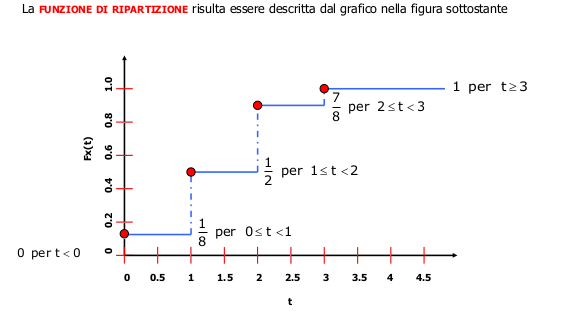
\includegraphics[scale=0.8]{img/rip.png}
\end{figure}
Avendo definito la funzione di ripartizione, adesso tutte le questioni riguardanti la variabile casuale $X$
possono trovare una soluzione attraverso di essa, infatti supponiamo di calcolare $P(\{a < X \leq b\})$
con l'evento ${X \leq b}$ esprimibile come l'unione dei due eventi indipendenti ${X \leq a}$ e ${a < X \leq b}$ 
da cui si ricava, usando il terzo assioma della probabilità la seguente formula:
\[ \begin{split}
        P(\{X \leq b\}) & = P(\{X \leq a\}) + P(\{a < X \leq b\}) \ \text{da cui si ricava} \\
        P(\{a < X \leq b\}) & = F(b) - F(a) \\
    \end{split} \]
Questa formula ci permette di determinare la probabilità che una variabile casuale possa assumere valori in intervalli reali
e ciò ha un notevole utilizzo in statistica e nella probabilità.

In genere la funzione di ripartizione non è nota, altrimenti tutti gli eventi della nostra vita sarebbero facilmente analizzabili
senza nessuna incertezza, ossia ad esempio si sarebbe in grado di prevedere come vincere al superenalotto e
tutti i giochi d'azzardo,  per cui l'obiettivo della statistica è di determinarla o determinare le grandezza ad essa associate
mentre la probabilità e le sue applicazioni assumono che essa sia  sempre nota.

Si dimostra che sono delle funzioni di ripartizione tutte e sole le funzioni del tipo $F: \R \to [0, 1]$
che godono simultaneamente delle seguenti proprietà:
\begin{itemize}
    \item $F$ è monotona crescente
    \item $\lim_{t \to +\infty} F(t) = 1$
    \item $\lim_{t \to -\infty} F(t) = 0$
    \item $\lim_{t \to t_0 ^ +} F(t) = F(t_0),\,\,\forall t_0 \in \R$
\end{itemize}
Le variabili aleatorie si distinguono in due categorie, in base a che valori può assumere 
l'insieme di valori $S$ di supporto:
\begin{itemize}
    \item \emph{variabili aleatorie discrete}: l'insieme $S$ è finito oppure costituito da un insieme
                                               infinito di valori discreti.
    \item \emph{variabili aleatorie continue}: l'insieme $S$ assume valori infiniti continui
\end{itemize}
Iniziamo ad analizzare prima le variabili discrete, più semplici da analizzare per poi considerare il caso
continuo, in cui si estendono i valori assumibili dalle variabili.

\subsection{Variabile Aleatoria Discreta}
Come già visto, una variabile aleatoria è detta \emph{variabile aleatoria discreta} nel caso in cui l'insieme dei valori $S$
che essa può assumere  è finita oppure da un infinito di valori discreti, in cui si associa anche, oltre alla
funzione di ripartizione, una funzione di probabilità assunta da valori specifici.\newline
Sia $S$ il supporto della variabile aleatoria $X$ e si definisce \emph{distribuzione discreta di probabilità} la funzione:
$p_X:\R \to [0,1]$ così definita:
\[
    p_X = \begin{cases}
            P(X = t)& \forall t \in S\\
            0& \mbox{ altrimenti}\\
          \end{cases}\]
Una funzione rappresenta una distribuzione di probabilità, in caso siano soddisfatte entrambe le seguenti proprietà:
\begin{itemize}
    \item \[ p_X(t) \geq 0 \quad \forall t \in R \]
    \item \[ \sum _{s \in S} p_X(s) = 1 \]
\end{itemize}
Tra le funzioni di ripartizione e le distribuzioni discrete esiste una corrispondenza biunivoca, in quanto
si hanno le seguenti equivalenze:
\begin{itemize}
    \item \[F_X(t) = \sum _{s \in S:s \subseteq t} p_X(s)\,\,\, \forall t \in \R\]
    \item \[p_X(s) = F_X(s) - \lim _{t \to s^{-}} F_X(t)\,\,\, \forall s \in S\]
\end{itemize}
Dalla prima di tali relazioni se ne deduce che le funzioni di ripartizione delle variabili
aleatorie discrete presentano dei \textit{salti} in corrispondenza dei valori \textit{s} mentre
sono costanti per gli altri valori, come si può anche notare nella figura ~\ref{img:ripartizione}

\subsection{Variabile Aleatoria Continua}
Come già affermato in precedenza, una variabile aleatoria è detta continua nel caso in cui la 
corrispondente funzione di ripartizione $F_X$ sia continua, ed in particolare viene detta 
\emph{assolutamente continua} se esiste una funzione $f_X:\R \to \R_+$ tale che
\[F_X(t) = \int _{-\infty}^t f_X(u)du \,\,\, \forall t \in \R\]
Una tale funzione, in caso in cui è definito l'integrale, viene detta \emph{densità di probabilità }di $X$.

È detto poi \emph{supporto} della variabile $X$ l'insieme $S = \{t \in \R : f_X(t) \neq 0\}$
e si osservi che se la densità di probabilità esiste allora la sua funzione di ripartizione è una sua
primitiva.

Per semplicità supporremo nel seguito che le variabili aleatorie assolutamente continue abbiano funzione
di ripartizione derivabile e che la funzione di densità di probabilità sia la derivata della funzione di ripartizione.\newline
Come anche per le distribuzioni discrete di probabilità, le funzioni di densità di probabilità 
per essere tali devono soddisfare le seguenti due proprietà:
\begin{enumerate}
    \item \[f_X(t) \geq 0\,\,\, \forall t \in \R\]
    \item \[\int _{-\infty}^{+\infty} f_X(t)dt = 1\]
\end{enumerate}
La probabilità che una variabile aleatoria continua (o assolutamente continua) assuma un ben determinato valore
è sempre nulla, in quanto se $X$ è una variabile aleatoria continua allora per ogni $t_0 \in R$ risulta
\[ \begin{split}
    P(X = t_0) & = P(X \leq t_0) - \lim _{t \to t_0^-} P(X \leq t) \\
               & = F_X(t_0) - \lim_{t \to t_0^-} F_X(t) \\
               & = F_X(t_0) - F_X(t_0) = 0\\
   \end{split} \]

\begin{figure}
    \centering
    \caption{Funzione di ripartizione continua}
    \label{img:ripartizioneContinua}
    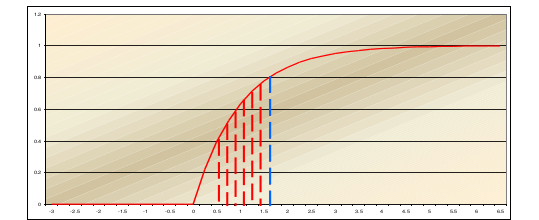
\includegraphics[scale=0.6]{img/con.png}
\end{figure}
Pertanto, quando si pensa a variabili aleatorie continue, non ha mai senso domandarsi quale sia la probabilità
che esse assumano valori esatti, ma conviene invece domandarsi quale è la probabilità che essi assumano
specifici valori appartenenti in specifici intervalli dell'asse reale.

Per calcolare la probabilità che una variabile casuale continua $X$ assuma un valore in un intervallo 
$(a,b] \subseteq \R$ è possibile far ricorso alla formula:
\[ P(X \in (a,b]) = \int _a ^b f_X(u)du\,\,\,  \text{da cui si ricava}\]
\[ \begin{split}
    P(X \in (a, b]) & = F_X(b) - F_X(a) \\
                    & = \int_{-\infty}^b f_X(u)du - \int_{-\infty}^a f_X(u)du\\
   \end{split} \]
In pratica la probabilità che sia soddisfatto l'evento $X\in(a,b]$ corrisponde all'area sottesa
dalla densità $f_X$ nell'intervallo $(a,b]$, come si può notare nella figura ~\ref{graficoRipartizione}, per cui

\begin{figure}
    \center
    \caption{Esempio di calcolo della densità di probabilità continua}
    \label{graficoRipartizione}

    \psscalebox{1.0 1.0} % Change this value to rescale the drawing.
{
\begin{pspicture}(0,-2.375)(8.38,2.375)
\psbezier[linecolor=black, linewidth=0.04](5.9990716,0.4275487)(5.9981446,1.2275481)(1.6000015,-0.37754923)(1.6009284,-1.1775487080233007)
\psline[linecolor=black, linewidth=0.04, arrowsize=0.05291667cm 2.0,arrowlength=1.4,arrowinset=0.0]{->}(0.8,-2.375)(0.8,2.425)
\psline[linecolor=black, linewidth=0.04, arrowsize=0.05291667cm 2.0,arrowlength=1.4,arrowinset=0.0]{->}(0.4,-1.975)(7.2,-1.975)
\psline[linecolor=black, linewidth=0.04, linestyle=dashed, dash=0.17638889cm 0.10583334cm](1.6,-1.175)(1.6,-1.975)
\psline[linecolor=black, linewidth=0.04, linestyle=dashed, dash=0.17638889cm 0.10583334cm](6.0,0.425)(6.0,-1.975)
\rput[bl](1.6,-2.375){$a$}
\rput[bl](5.6,-2.375){$b$}
\rput[bl](7.2,-2.375){$X$}
\rput[bl](-0.1,2.025){$f_X()$}
\rput[bl](6.4,-0.775){$P(X\in(a,b])$}
\psline[linecolor=black, linewidth=0.04, linestyle=dotted, dotsep=0.10583334cm](5.6,0.425)(2.0,-1.175)
\psline[linecolor=black, linewidth=0.04, linestyle=dotted, dotsep=0.10583334cm](5.6,0.025)(2.0,-1.575)
\psline[linecolor=black, linewidth=0.04, linestyle=dotted, dotsep=0.10583334cm](5.6,-0.375)(2.0,-1.975)
\psline[linecolor=black, linewidth=0.04, linestyle=dotted, dotsep=0.10583334cm](5.6,-0.775)(2.8,-1.975)
\psline[linecolor=black, linewidth=0.04, linestyle=dotted, dotsep=0.10583334cm](5.6,-1.175)(3.6,-1.975)
\psline[linecolor=black, linewidth=0.04, linestyle=dotted, dotsep=0.10583334cm](5.6,-1.575)(4.8,-1.975)
\end{pspicture}
}

\end{figure}

\[[P(X\in(a,b]) = \int_a^bf_X(u)du\,\,\,\forall a,b \in \R,\,\,\,a<b\]
Essendo inoltre $P(X = a) = 0$ si ha:
\[ P(X \in (a, b]) = P(X\in[a,b])\,\,\,\forall a,b \in \R,\,\,\,a<b\]
Si ha che la funzione di ripartizione è la funzione integrale della funzione di densità di probabilità,
quindi si ottiene la funzione di densità di probabilità tramite derivazione:
\[\frac{d}{dt} F_X(t) = f_X(t)\]

\subsection{Variabili Aleatorie Multidimensionali}
In molti casi è lecito considerare situazioni (esperimenti) il cui esito è rappresentato, 
anziché da un valore numerico, da una coppia o da una n-pla di valori, in tal caso 
si parla di \textit{variabili aleatorie multidimensionali}.\newline
Anche qui le variabili sono definite da uno spazio campione $\Omega$ a $\R^n$, con $n$ dimensione della variabile,
ed è comodo pensare a queste variabili aleatorie come a risultati esprimibili da n-ple di valori numerici.\newline
Consideriamo quindi le \emph{variabili aleatorie bidimensionali assolutamente continue}, 
anche se ovviamente si può estendere a $n$ variabili anche non continue.

Sia quindi una variabile aleatoria $(X, Y): \Omega \to \R ^ 2$ con $\Omega$, uno spazio campione 
al quale è associata una probabilità $P$ definita sui sottoinsiemi di $\Omega$.\newline
Si definisce la \emph{funzione di ripartizione congiunta} la funzione bidimensionale 
$F_{X, Y}(t, s):\R ^2 \to [0,1] \subseteq \R$ definita come:
\[F_{X, Y} = P(\{X \leq t\} \cap \{Y \leq s\}\,\,\,\forall (t,s)\in \R\]
inoltre se la variabile $(X,Y)$ è assolutamente continua esiste la \emph{funzione dei densità congiunta}
$f_{X, Y}:\R ^2 \to \R_+$ tale che
\[F_{X, Y}(t, s) = \int_{-\infty}^t \int_{-\infty}^s f_{X, Y}(u, v)du\,dv\,\,\,\forall (t, s)\in \R ^2\]
Conoscendo una delle due funzioni sopra è possibile determinare la probabilità che la coppia $(X,Y)$ assuma
valori in un qualsiasi sottoinsieme rettangolare $(a_1, b_1] \times (a_2, b_2] \in \R^2$, in cui risulta:
\[ \begin{split}
    P((X, Y) \in (a_1, b_1] \times (a_2, b_2]) & = F_{X, Y} (b_1, b_2) - F_{X, Y}(a_1, b_2)\\ 
                                               & - F_{X, Y} (b_1, a_2) + F_{X, Y}(a_1, a_2) \\
    & = \int_{a_1}^{b_1} \int_{a_2}^{b_2} f_{X, Y}(u, v) du\,dv\,\,\, \forall (a_1, b_1] \times(a_2, b_2] \in \R^2\\
   \end{split}\]

\begin{figure}
    \caption{Densita di probabilità multidimensionale}
    \label{img:densitaMulti}
    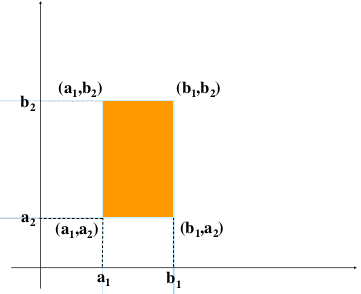
\includegraphics[scale=0.7]{img/mul.png}
\end{figure}
In molti casi, benché ci si trovi di fronte a situazioni i cui esiti sono di tipo multidimensionale, 
capita di essere interessati ai valori che possono essere assunti solamente da una delle variabili per cui 
sono state introdotte le \emph{funzioni marginali}.

Data una variabile aleatoria bidimensionale $(X, Y)$ assolutamente continua, avente 
funzione di ripartizione congiunta $F_{X, Y}$ e funzione di densità disgiunta $f_{X, Y}$ è detta 
\emph{funzione di ripartizione marginale di X} in caso si ha
\[ \begin{split}
    F_X(t) & = P(\{X \leq t\} \cap \{Y \leq +\infty\})\\
           & = F_{X, Y}(t, +\infty)\\
   \end{split}\]
mentre si definisce la funzione p detta \emph{funzione di densità marginale di X} come
\[f_X(t) = \int_{-\infty}^{+\infty} f_{X, Y}(t, s)\,ds\]
Data una variabile bidimensionale $(X, Y)$ diciamo che le due variabili considerate singolarmente 
sono \emph{stocasticamente indipendenti} se e solo se per ogni $(t, s) \in \R^2$ vale
\[F_{X, Y}(t, s) = F_X(t) \cdot F_Y(s)\]
che discende dalla definizione di stocasticamente indipendente fornita nella teoria assiomatica della probabilità.

\section{Indici delle variabili aleatorie}
Iniziamo ad affrontare gli indici associati alle variabili aleatorie, partendo prima dagli indici centrali,
grandezze numeriche associate alle variabili aleatorie, in grado di sintetizzare, con un solo valore,
le principali caratteristiche delle loro distribuzioni.\newline
Gli indici risultano strettamente legati agli indici introdotti nella prima parte in relazione alla 
statistica descrittiva, il più importante degli indici di tendenza centrale è detto \emph{valore atteso}
corrispondente alla media matematica dei dati statistici.

Data una variabile aleatoria unidimensionale $X$ avente supporto $S \subseteq \R$ è detto valore atteso di $X$ la quantità:
\[E[X] = \begin{dcases}
           \sum_{s\in S}\,\, s\cdot p_X(s) \,\,\mbox{ se X è discreta}\\
           \int_{-\infty}^{+\infty}\,\, u\cdot f_X(u)\,du \,\,\mbox{ se X è assolutamente continua}\\
         \end{dcases}\]
In effetti il valore atteso, così come la media di una serie di dati, va pensato come una \textit{media pesata}
dei valori assumibili dalla variabile, e fornisce un'indicazione di massima del posizionamento della variabile
lungo l'asse dei numeri reali.\newline
Il valore atteso gode delle seguenti tre proprietà:
\begin{enumerate}
    \item $\forall a \in \R$, se $X = a$ con probabilità uguale ad 1, allora $E[X] = a$
    \item $E[a\cdot X + b] = a\cdot E[X] + b$ per ogni variabile $X$ e per ogni $a, b \in \R$
    \item data una funzione $y = g(X)$ della variabile aleatoria $X$ si ha che il valore atteso è:
            \[E[g(X)]=\int_{-\infty}^{+\infty}g(u)f_X(u)\,du\]
\end{enumerate}
Il valore atteso non è detto che esista, infatti in caso l'integrale o la sommatoria non convergono il valore
atteso risulta non definito e come avevamo già visto con la media, il valore atteso è in realtà un caso
particolare di momento centrale di ordine $r = 1$, la cui formula è definita come:
\[ E[X^r] = \begin{dcases}
                \sum _{s \in S} \,\, s^r \cdot p_X(s) \,\,\mbox{se X è discreta}\\
                \int_{-\infty}^{+\infty}\,\, u^r\cdot f_X(u)\,du \,\,\mbox{ se X è assolutamente continua}\\
            \end{dcases}\]
Un altro indice di tendenza centrale importante è la \emph{moda} di una variabile aleatoria $X$, indicata
con $\widetilde{X} \in \R$, corrispondente al valore per cui è massima la distribuzione discreta di
probabilità, se $X$ è discreta, oppure rappresenta la funzione di densità; tale valore non è detto che sia
unico, ma può avere la presenza di più valori di moda, e ciò porta a parlare di distribuzione multimodale.

Un terzo indice di tendenza centrale è la \emph{mediana}  di una variabile aleatoria $X$, 
indicata con $\hat{X} \in \R$, che soddisfa la diseguaglianza:
\[ \lim_{t \to \hat{X}^-} F_X(t) \leq \frac{1}{2} \leq F_X(\hat{X})\]
Nel caso in cui la funzione di ripartizione della variabile sia continua ed invertibile allora:
$\hat{X}=F_X^{-1}(\frac{1}{2})$ mentre nel caso di variabili discrete la mediana è il valore dell'ascissa
in cui la funzione di ripartizione passa da un valore minore di $\frac{1}{2}$ ad uno superiore.\newline
La mediana può non essere unica, e ciò avviene in caso esistano più valori $t$ per cui risulta $F_X(t) = \frac{1}{2}$.

\begin{figure}
    \centering
    \caption{grafico di moda, mediana e media}
    \label{fig:centralValue}
    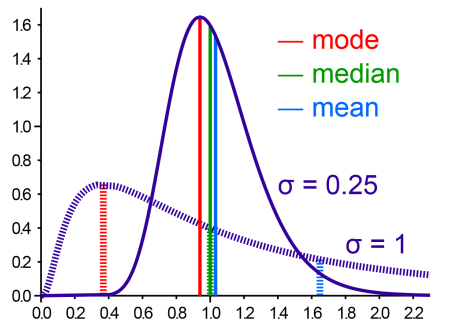
\includegraphics[scale=0.7]{img/mmm.png}
\end{figure}
Unitamente alla mediana è possibile considerare altri indici definiti in maniera simile e che dividono
la retta dei reali in due intervalli di probabilità assegnata e che sono detti \emph{quantili}, come si nota
nella \figurename~\ref{fig:quantile}.
Dato un valore $P \in [0,1] \subseteq \R$ è detto \emph{quantile p-esimo della variabile aleatoria X} il valore
$x_p \in \R$ tale che
\[ \lim_{t \to x_p^{-}} F_X(t) \leq p \leq F_X(x_p)\]
Nel caso in cui la funzione di ripartizione sia continua ed invertibile, allora $x_p = F_X^{-1}(p)$
e questa definizione ci porta a pensare a $x_p$ come ad un valore in cui risulta 
$P(X \leq x_p) = p$ e $P(X > x_p) = 1-p$.

\begin{figure}
    \centering
    \caption{Grafico del quantile}
    \label{fig:quantile}
    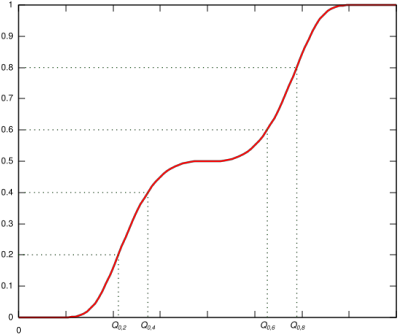
\includegraphics[scale=0.5]{img/qua.png}
\end{figure}

Come visto in precedenza, nella statistica descrittiva, oltre agli indici di tendenza centrale è conveniente 
anche considerare indici che forniscano un'idea del grado di dispersione dei valori 
assumibili da una variabile aleatoria.\newline
Questi vengono detti \emph{indici di variabilità}: il più famoso tra tutti è la \emph{varianza}
di una variabile aleatoria $X$, indicata con $\sigma_X ^ 2$, definita come:
\[V[X] = \begin{dcases}
            \sum_{s \in S}\,\, (s - E[X])^2 \cdot p_X(s)\mbox{ se X è discreta}\\
            \int_{-\infty}^{+\infty}\,\, (u - E[X])^2 \cdot f_X(u)\,du\mbox{ se X è assolutamente continua}\\
         \end{dcases}\]
Così come il valore atteso anche la varianza talvolta può non esistere, quando la sommatoria o l'integrale divergono.\newline
La radice della varianza è anch'esso un altro indice importante, detto \emph{deviazione standard}, il cui
vantaggio rispetto alla varianza è quello di avere la stessa unità di misura del valore atteso.

La varianza ha le seguenti proprietà:
\begin{enumerate}
    \item $\forall a \in \R$, se $X = a$ con probabilità uguale ad 1 allora $V[X] = 0$
    \item $V[a\cdot X + b] = a^2 \cdot V[X] + b$ per ogni variabile $X$ e per ogni $a,b \in \R$
    \item $V[X] = E[X^2] - (E[X])^2\,\,\forall X$ variabile aleatoria
\end{enumerate}
Anche per le variabili multidimensionali ed in particolare per quelle bidimensionali 
esistono indici di tendenza centrale e variabilità.\newline
Sia $(X, Y)$ una variabile aleatoria bidimensionale discreta o continua, sono detti \emph{valori attesi marginali} 
e \emph{varianza marginali }le quantità $E[X]\,\,E[Y]\,\,V[Y]\,\,V[Y]$
ottenute considerando le distribuzioni marginali di $X$ ed $Y $ ed integrando (o sommando) in accordo ai sistemi visti sopra.

Si hanno le seguenti relazioni:
\begin{itemize}
    \item $E[a\cdot X + b \cdot Y] = a\cdot E[X] + b\cdot E[Y]\,\,\forall \mbox{ coppia }X,Y \mbox{ e }
                                     \forall a,b \in \R$
    \item $E[X \cdot Y] = E[X]\cdot E[Y]\,\,\mbox{per ogni coppia }X,Y \mbox{ stocasticamente indipendenti}$
    \item $V[X + Y]= V[X] + V[Y]\,\, \mbox{ per ogni coppia }X,Y \mbox{ stocasticamente indipendenti}$
\end{itemize}
Oltre ai valori attesi ed alle varianze marginali, un altro indice estremamente importante, 
è la \textbf{covarianza} definita come:
\[ \begin{split}
    Coc[X, Y] & = E[(X-E[X])\cdot(Y-E[X])]\\ 
              & = \iint_{\R^2} (t - E[X])\cdot (s - E[Y])\cdot f_{X,Y}(t,s)\,dt\,ds\\
              & = \iint_{\R^2} t \cdot s\cdot f_{x,y}(t,s)\,dt\,ds 
                  - \int_{\R} t \cdot f_X(t) dt \cdot \int_{\R}s \cdot f_Y(s)dt \\
    \end{split} \]
La covarianza è un indice della correlazione che sussiste tra due variabili ovvero del loro grado di
dipendenza reciproca, in cui tanto essa è grande quanto è forte il legame di dipendenza tra le variabili.

In caso la covarianza è nulla le due variabili aleatorie vengono dette \textbf{incorrelate}, relazione 
meno forte della indipendenza stocastica, come avevamo già notato nel capitolo sulla statistica descrittiva.

Un ultimo indice è quello detto \emph{coefficiente di correlazione di Pearson}, strettamente legato 
alla covarianza ed utilizzato per esprimere più chiaramente il grado di dipendenza tra due variabili:
\[p_{XY} = \frac{Cov[X,Y]}{\sqrt{V[X]\cdot V[Y]}} = \frac{Cov[X,Y]}{\sigma_x\cdot \sigma_y}\]
questo indice ha le seguenti proprietà:
\begin{enumerate}
    \item $p_{XY}=0$ se $X$ e $Y$ sono incorrelate
    \item $|p_{XY}|=1$ se vale la relazione $Y= aX + b\,\,\,\forall a,b \in \R$
\end{enumerate}
Ovvero se vale $+1$ allora $a>0$ e se vale $-1$ si ha che $a<0$.

\section{Esercizi}
\begin{esercizio}
2 carte con reintroduzione si estraggono da un mazzo da 52.
\begin{enumerate}

\item P che prima sia di picche seconda di quadri
\item P di due figure dello stesso seme
\item se la prima è > 4 calcolo P che la seconda sia 10

\end{enumerate}
risposte:
\begin{enumerate}

\item P1 prima carta picche e Q2 seconda carta quadri. Sono eventi indipendenti per la reintroduzione
\[P(P1\cap Q2)=P(P1)\cdot P(Q2)=\frac{13}{52}\cdot \frac{13}{52}=\left(\frac{13}{52}\right)^2\]
\item A carta di seme X e B carta di seme X, si ricorda reintroduzione
\[P(A\cap B)=P(A)\cdot P(B|A)=\frac{12}{52}\cdot \frac{3}{52}= \frac{9}{876}\]
\item C carta > 4 e D carta = 10, la carta è sempre la stessa
\[P(D|C)=\frac{P(D\cap C)}{P(C)}=\frac{P(D)}{P(C)}=\frac{1}{9}\]
\end{enumerate}
\end{esercizio}
\begin{esercizio}
Gli abitanti di abc raggiungono xyz col treno con con la macchina. Il 90\% arriva in ritardo, il 40\% di questi usa il treno. Il 20\% di quelli che non arriva in ritardo usano la macchina.
\begin{enumerate}
\item probabilità che un abitante usi il treno
\item se usa il treno percentuali di ritardo o meno
\end{enumerate}
risposte
\begin{enumerate}
\item R = 0.9 persona in ritardo, $\overline{R}=0.1$ non in ritardo, T usa treno e M usa macchina\\
\[P(T)=P(R)\cdot P(T|R)+P(\overline{R})\cdot P(T|\overline{R})=0.9*0.4+0.1*0.8=0.44\]
\item \[P(R|T)=\frac{P(R\cap T)}{P(T)}=\frac{P(T|R)\cot P(R)}{P(T)}=\frac{0.9*0.4}{0.44}=0.8182\]
quindi per la macchina è $1-0.8182=0.1818$
\end{enumerate}
\end{esercizio}
\begin{esercizio}
Un urna contiene una pallina rossa e una bianca, ne estraggo una e la rimetto dentro con un'altra dello stesso colore. All'i-sima estrazione se ne estrae una rossa (Ri) e all'i-esima estrazione una bianca(Bi)
\begin{enumerate}
\item P(R2) alla seconda estrazione una rossa e P(R3) alla terza estrazione una rossa
\item se la seconda è rossa la prima era più probabile bianca o rossa?
\item P di avere prima rossa e seconda bianca
\end{enumerate}
risposta:
\begin{enumerate}
\item \[P(R2)=P(R1\cap R2)+P(B1\cap R2)=\]
\[P(R1\cap R2)=P(R1)\cdot P(R2|R1)= \frac{1}{2}\cdot \frac{2}{3}=\frac{1}{3}\]
\[P(B1\cap R2)=P(B1)\cdot P(R2|B1)=\frac{1}{2}\cdot \frac{1}{3}=\frac{1}{6}\]
\[P(R2)=\frac{1}{2}\]
\[P(R3)=P(R1\cap R2\cap R3)+P(R1\cap B2\cap R3)+P(B1\cap R2\cap R3)+P(B1\cap B2\cap R3)\]
\[P(R1\cap R2\cap R3)=P(R1)\cdot P(R2|R1)\cdot P(R3|R1\cap R2)=\frac{1}{2}\cdot \frac{2}{3}\cdot \frac{3}{4}=\frac{1}{4}\]
\[P(R1\cap B2\cap R3)=P(R1)\cdot P(B2|R1)\cdot P(R3|R1\cap B2)=\frac{1}{2}\cdot \frac{1}{3}\cdot \frac{1}{2}=\frac{1}{12}\]
\[P(B1\cap R2\cap R3)=P(B1)\cdot P(R2|R1)\cdot P(R3|R1\cap R2)=\frac{1}{2}\cdot \frac{1}{3}\cdot \frac{1}{2}=\frac{1}{12}\]
\[P(B1\cap B2\cap R3)=P(B1)\cdot P(B2|R1)\cdot P(R3|R1\cap B2)=\frac{1}{2}\cdot \frac{2}{3}\cdot \frac{1}{4}=\frac{1}{12}\]
\[P(R3)=\frac{1}{4}+\frac{1}{12}+\frac{1}{12}+\frac{1}{12}=\frac{1}{2}\]
\item \[P(R1|R2)=\frac{P(R1\cap R2}{P(R2)}=\frac{P(R1)\cdot P(R2|R1}{P(R2)}=\frac{\frac{1}{2}\cdot \frac{2}{3}}{\frac{1}{2}}=\frac{2}{3}\]
\[P(B1|R2)=\frac{P(B1\cap R2}{P(R2)}=\frac{P(B1)\cdot P(R2|B1}{P(R2)}=\frac{\frac{1}{2}\cdot \frac{1}{3}}{\frac{1}{2}}=\frac{1}{3}\]
\item \[P(R1\cap B2)=P(R1)\cdot P(B2|R1)=\frac{1}{2}\cdot \frac{1}{3}=\frac{1}{6}\]
\end{enumerate}
\end{esercizio}

\chapter{Distribuzioni Notevoli}
Essendoci una correlazione, come notato nel precedente capitolo, tra la funzione di ripartizione e
la sua distribuzione/densità di probabilità, si parla di \textbf{distribuzione} di una variabile
intentendo indifferentemente la sua ripartizione o la sua densità/distribuzione.\newline
Con $X \sim F$ si indica che la variabile $X$ è distribuita secondo la distribuzione $F$.

Adesso affrontiamo una serie di distribuzioni famose, che hanno un notevole successo ed utilizzo in campo
statistico e probabilistico, incominciando dalle distribuzioni discrete e poi si analizzano quelle assolutamente continue.

\section{Distribuzioni discrete}
Le distribuzioni discrete maggiormente utilizzate sono le seguenti:
\begin{itemize}
    \item bernoulliana
    \item binomiale
    \item poisson
    \item geometrica
\end{itemize}
Una variabile aleatoria X è detta distribuita secondo una Bernoulliana di parametro $p\in[0,1]$, indicata con
$X \sim B(p)$ se essa può assumere solo i valori 1 e 0 rispettivamente con probabilità $p$ e $(1 - p)$.\newline
Questa distribuzione presenta le seguenti funzioni di ripartizione e la sua corrispondente distribuzione di probabilità:
\begin{itemize}
    \item $p_X(t) = \begin{cases}
                    1 - p \mbox{ se } t = 0\\
                    p     \mbox{ se } t = 1\\
                    0     \mbox{ altrimenti}\\
                    \end{cases}$
    \item $F_X(t) = \begin{cases}
                    0     \mbox{ se } t < 0\\
                    1 - p \mbox{ se } 0 \leq t < 1\\
                    1     \mbox{ se } t \geq 1\\
                    \end{cases}$
\end{itemize}
L'importanza di questa semplice distribuzione è ovvia, in quanto sono variabili di Bernoulli tutte quelle
che individuano il verificarsi di uno specifico evento e che valgono 1 se questo si verifica e 0 altrimenti.

Attraverso l'applicazione della definizione di valore atteso e di varianza si ottiene:
    \[ E[X] = 0 \cdot (1-p) + 1\cdot p = p\]
    \[ V[X] = [0^2 \cdot (1-p) + 1^2 \cdot p] = (1-p) \cdot p\]

Siano $X_1, \cdots, X_n \,  n$ variabili Bernoulliane di identico parametro $p$ e stocasticamente indipendenti tra loro,
e sia anche $X = \sum X_i$, variabile definita distribuita secondo una binomiale di parametri $n$ e $p$,
espressa con $X \sim Bin(n, p)$, se tale variabile può assumere qualsiasi valore intero $k$ compreso tra 0 e $n$,
in accordo con la seguente probabilità:
\[ P(X = k) = \binom{n}{k} \cdot p^k \cdot (1 - p) ^{n-k} \]
La parte $p^k \cdot (1-p)^{n - k}$ fornisce la probabilità che $k$ delle n variabili $X_i$ assumano il valore 1
e che le restanti $n - k$ variabili assumano valore 0 mentre la prima parte $\binom{n}{k}$, come ovvio dal
corso di matematica discreta, fornisce il numero  di combinazioni possibili delle variabili $k$.

In questa distribuzione vengono definite le seguenti funzioni di ripartizione e di distribuzione:
\begin{itemize}
    \item \[p_X(t) = \begin{dcases}
                        \binom{n}{t} p^t (1-p)^{n-t} \mbox{ se } t \in \{0,\cdots, n\}\\
                        0 \mbox{ altrimenti }\\
                     \end{dcases} \]
    \item \[F_X(t) = \sum_{0 \leq k \leq n; k\leq t} \binom{n}{k} p^k (1-p) ^{n - k},\,\,\forall t \in \R\]
\end{itemize}
Le variabili $X_i$ sono indipendenti quindi posso calcolare il valore atteso e la varianza di $X$:
\[E[X] = E[X_1 + \cdots + X_n] = E[X_1] + \cdots + E[X_n] = n \cdot p\]
\[V[X] = V[X_1 + \cdots + X_n] = V[X_1] + \cdots + V[X_n] = n \cdot (1-p) \cdot p\]
La principale applicazione della distribuzione binomiale consiste nella definizione di variabili che "contano" le 
realizzazioni di eventi quando questi siano da considerarsi indipendenti e con identica probabilità di verificarsi.

\begin{figure}
    \caption{Distribuzione binomiale}
    \label{fig:binomiale}
	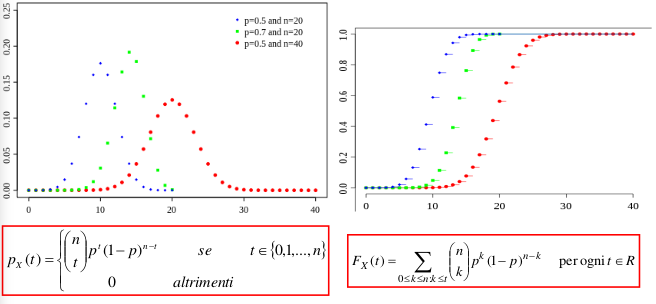
\includegraphics[scale=0.7]{img/dis5.png}
\end{figure}
La distribuzione di Poisson può essere vista come un caso particolare della distribuzione Binomiale 
che si ottiene quando il numero di variabili $X_i$ che compaiono in $X = \sum X_i$ tende ad infinito 
mentre il valore del parametro $p$ tende a zero, in modo tale che il prodotto $\lambda = n\cdot p$ resti costante. 

In caso ciò viene rispettato definiamo $X$ distribuita secondo una Poisson con parametro $\lambda \in \R_+$,
indicata con $X \sim Poi(\lambda)$, applicabile sui valori in $\R$.\newline
La probabilità associata a questa distribuzione è la seguente:
\[ P(X = k) = \lim_{n \to +\infty} \binom{n}{k} \cdot p^k \cdot (1-p)^{n-k} = \frac{\lambda^k}{k!} 
                                                                              e^{-\lambda} \,\, \forall k \in \N\]
la \textit{distribuzione di probabilità} e la \textit{funzione di ripartizione} risultano essere quindi:
\[p_X(t) = \begin{dcases}
           \frac{\lambda^k}{k!} e^{-\lambda} \mbox{ se } t \in \{0,\cdots, n\}\\
           0                                 \mbox{ altrimenti}\\
           \end{dcases}\]
        \[F_X(t) = \sum_{k \in \N:k \leq t} \frac{\lambda^k}{k!} e^{-\lambda},\,\,\forall t \in \R \]
valore atteso e varianza le ricavo da quelli delle bernoulliane con $\lambda = n\cdot p$:
\[E[X] = n \cdot p = \lambda\]
\[V[X] = n \cdot (1-p) \cdot p = n \cdot p-n \cdot p^2 = \lambda-\frac{\lambda^2}{n}\]
che con $n \to +\infty$ diventa $V[X] = \lambda$.

La distribuzione di Poisson viene utilizzata quando si considerino grandi popolazioni di individui in cui 
ogni individuo ha una probabilità p molto piccola di essere soggetto ad uno specifico evento in esame;
per tale ragione la distribuzione di Poisson viene anche detta degli eventi rari.
\begin{figure}
    \caption{Distribuzione di Poisson}
    \label{fig:poisson}
	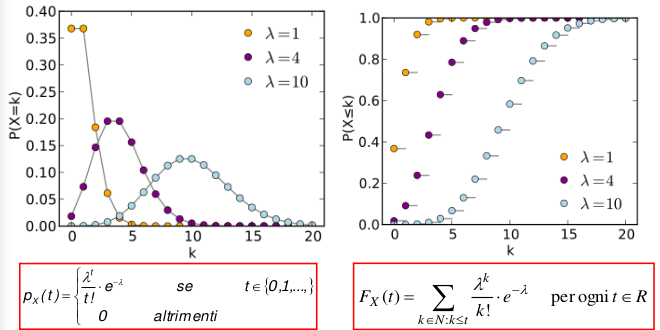
\includegraphics[scale=0.7]{img/dis4.png}
\end{figure}

Una variabile aleatoria X è detta distribuita secondo una Geometrica di parametro $p\in[0,1]$, indicata con $X \sim Geo(p)$,
se può assumere qualsiasi valore intero non negativo k con probabilità $P(X = k) = p \cdot (1-p)^k$.

La distribuzione di probabilità e la funzione di ripartizione risultano essere quindi:
\[p_X(t) = \begin{cases}
            p \cdot (1-p)^t \mbox{ se } t \in \N\\
            0               \mbox{ altrimenti}\\
           \end{cases}\]
\[F_X(t) = \sum_{k \in \N:k \leq t} p \cdot (1-p)^k,\,\,\forall t \in \R\]
con valore atteso e varianza:
\[E[X] = \frac{1-p}{p}\]
\[V[X] = \frac{1-p}{p^2}\]
Questa distribuzione ha la proprietà di \textbf{assenza di memoria}, ossia risulta $P(X = k + m | X \geq m) = P(X = k)$. 

Per comprenderne il significato, supponiamo che X sia il tempo di vita di una macchina soggetta a guasti
, che possono avvenire solo in corrispondenza di intervalli di tempo unitari, e supponiamo di aver rilevato
che per m unità di tempo essa non si sia guastata.\newline
La proprietà di assenza di memoria asserisce che la probabilità che la macchina si guasti all'istante $(k+m)$-esimo,
condizionata dall'evento $X \geq m$, è uguale alla probabilità iniziale che essa si guasti all'istante k-esimo.\newline
Quindi questa proprietà asserisce che il tempo trascorso da quando abbiamo iniziato ad esaminare il funzionamento
della macchina non influisce sulla distribuzione del tempo restante al verificarsi del guasto.

\section{Distribuzioni continue}
Le distribuzioni continue, affrontate in questo corso sono le seguenti:
\begin{itemize}
    \item uniforme
    \item triangolare
    \item esponenziale
    \item normale(o gaussiana)
\end{itemize}
Parliamo ora della \emph{distribuzione uniforme}, che rappresenta la più semplice distribuzione assolutamente continua
e viene adottata nel caso in cui la variabile considerata possa assumere qualsiasi valore compreso
in un dato intervallo con probabilità costante.\newline
Si dice che la variabile $X$ è distribuita secondo una uniforme di supporto $[a,b]$, indicata con $X \sim U[a, b]$
se essa è assolutamente continua con densità e funzione di ripartizione:
\[f_X(t) = \begin{dcases}
            \frac{1}{b-a} \mbox{ se } t \in [a,b]\\
            0             \mbox{ altrimenti}\\
           \end{dcases}\]
\[F_X(t) = \begin{dcases}
            0 \mbox{ se } t < a\\
            \frac{t-a}{b-a} \mbox{ se } t \in [a,b]\\
            1 \mbox{ se } t > b\\
            \end{dcases}\]
e con semplici integrazioni è possibile ricavare il valore atteso e la varianza:
\[E[X] = \frac{a+b}{2}\]
\[V[X] = \frac{(b-a)^2}{12}\]
Come accennato in precedenza l'interesse in questa distribuzione è giustificato dal fatto che essa descrive bene
situazioni nelle quali le variabili possono assumere valori in intervalli finiti di $\R$ con probabilità uniforme,
ovvero tale da essere identica per intervalli di medesima ampiezza, purchè contenuti nel supporto della variabile stessa.
\begin{figure}
    \caption{Distribuzione Uniforme}
    \label{img:uniforme}
	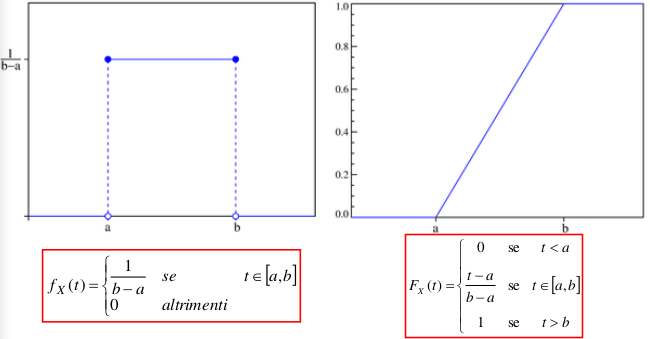
\includegraphics[scale=0.7]{img/dis2.png}
\end{figure}

Ovviamente non è certo che i valori assumibili abbiano tutti la stessa probabilità di presentarsi, per questo
sono stati introdotti alcune generalizzazioni della distribuzione uniforme;una di queste è la
\textbf{distribuzione triangolare}, che assegna alla densità di probabilità valori maggiori al centro del
supporto e minori in prossimità degli estremi.\newline
Formalmente diciamo che la variabile $X$ è distribuita secondo una Triangolare di supporto $[a,b]$, indicata
con $X \sim T[a, b]$ se essa è assolutamente continua con le seguenti funzioni di densità e ripartizione:
\[f_X(t) = \begin{dcases}
            \frac{4(t-a)}{(b-a)^2} \mbox{ se } t \in \left[a,\frac{a+b}{2}\right)\\
            \frac{4(b-t)}{(b-a)^2} \mbox{ se } t \in \left[\frac{a+b}{2},b\right]\\
            0                      \mbox{ altrimenti}
            \end{dcases}\]
\[F_X(t) = \begin{dcases}
            0 \mbox{ se } t<a\\
            \frac{2(t-a)^2}{(b-a)^2} \mbox{ se } t \in \left[a, \frac{a+b}{2}\right)\\
            1-2\frac{(b-t)^2}{(b-a)^2} \mbox{ se } t \in \left[\frac{a+b}{2}, b\right]\\
            1 \mbox{ se } t>b\\
            \end{dcases}\]
Attraverso l'integrazione delle funzioni presentate si ottiene il valore atteso e la varianza:
\[E[X] = \frac{a+b}{2}\]
\[V[X] = \frac{(b-a)^2}{24}\]

Passiamo alla \textbf{distribuzione esponenziale}, importante nello studio di variabili che descrivono i tempi
necessari per il verificarsi di un evento.\newline
Formalmente, una variabile aleatoria $X$ è distribuita secondo una Esponenziale di parametro $\lambda \in \R$,
indicata con $X \sim Exp(\lambda)$ se essa è assolutamente continua con le seguenti funzioni:
\[f_X(t) = \begin{dcases}
            \lambda e^{-\lambda t} \mbox{ se } t \geq 0\\
            0 \mbox{ altrimenti}
            \end{dcases}\]
\[F_X(t) = \begin{dcases}
            1 - e^{-\lambda t} \mbox{ se } t \geq 0\\
            0 \mbox{ altrimenti}
            \end{dcases}\]
Attraverso integrazione si ottengono valor medio e varianza:
\[E[X] = \frac{1}{\lambda}\]
\[V[X] = \frac{1}{\lambda^2}\]
L'importanza della distribuzione esponenziale in numerosi campi applicativi è dovuta al fatto che essa è
l’unica distribuzione assolutamente continua che gode della \textbf{proprietà di assenza di memoria}, vista
anche nella distribuzione geometrica, di tipo discreto.
\begin{figure}
    \caption{Distribuzione esponenziale}
	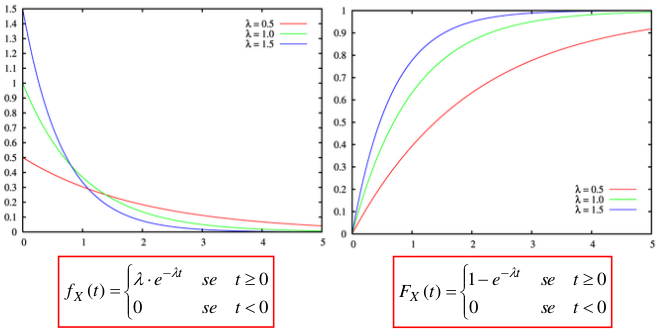
\includegraphics[scale=0.7]{img/dis.png}
\end{figure}
\subsection{Distribuzione Normale}
Una variabile aleatoria X è detta \emph{distribuita secondo una Normale con parametri} $\mu \in \R$ e $\sigma \in \R_+$,
indicata attraverso $X \sim N(\mu, \sigma)$, se essa è assolutamente continua con densità:
\[f_X(t)=\frac{1}{\sqrt{2\cdot \pi\cdot \sigma^2}}\cdot e^{-\frac{(t-\mu)^2}{2\cdot \sigma^2}}\,\,\,\forall t\in\R\]
Questa distribuzione è fondamentale per il \emph{teorema centrale del limite}, studiata nel prossimo
capitolo e poi perchè molti fenomeni studiati dalla statistica e dalla probabilità si comportano come una
normale, chiamata anche \emph{gaussiana}.

Integrando si ottengono il valore atteso e la varianza:
\[E[X] = \mu\]
\[V[X] = \sigma^2\]
\begin{figure}
    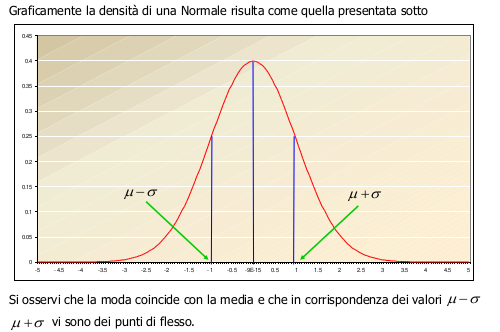
\includegraphics[scale=0.7]{img/norm.png}
\end{figure}
\begin{figure}
    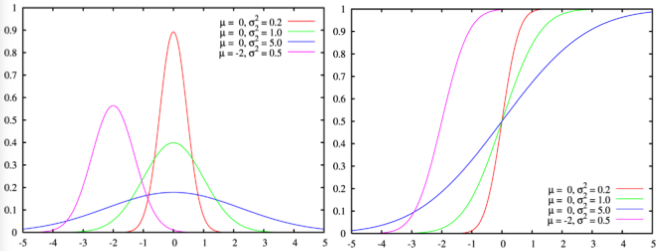
\includegraphics[scale=0.7]{img/nomr2.png}
\end{figure}
Calcolare la probabilità P, assunta da una variabile $X$ in un intervallo $[a, b]$ è notevolmente difficile in
quanto si deve risolvere la seguente equazione:
\[P(X \in [a,b]) = \int_a^b \frac{1}{\sqrt{2\cdot \pi\cdot \sigma^2}}\cdot e^{-\frac{(t-\mu)^2}{2\cdot \sigma^2}}\,dt\]
Per questa ragione si ricorre ad opportune tavole che si riferiscono alla distribuzione normale standard 
ovvero con parametri $\mu = 0$ e $\sigma = 1$ e che forniscono i valori di $\int_0^z f_X(t)\,dt$ 
per un elevato numero di valori $z \in \R$.\newline
Quando si sia interessati a determinare delle probabilità associate ad una generica normale ci si riconduce al
caso sopra osservando che la variabilie $Z = \frac{X - \mu}{\sigma}$ è distribuita secondo una \emph{Normale Standard}
\[\mbox{se } X \sim N(\mu, \sigma) \mbox{ allora } Z = \frac{X \mu}{\sigma} \sim N(0,1)\]
quindi ogni variabile $X \sim N(\mu, \sigma)$ può essere ricondotta ad una può essere ricondotta ad una Normale
standarizzata ovvero ancora per ogni ovvero ancora $\forall [a,b] \subseteq \R$ si avrà:
\[P(X \in [a,b]) = P(a \leq X \leq b) =P \left(\frac{a - \mu}{\sigma} \leq \frac{X-\mu}{\sigma} \leq 
                   \frac{b-\mu}{\sigma}\right) = P \left(Z \in \left[\frac{a-\mu}{\sigma},\frac{b-\mu}{\sigma}\right]\right)\]

La distribuzione gaussiana possiede la seguente proprietà:
\begin{definizione}
     $\mbox{se } X_1 \sim N(\mu_1,\sigma_1) \mbox{ e } X_2 \sim N(\mu_2, \sigma_2)$ e se $X_1$ e $X_2$
        sono indipendenti allora la variabile $Y = X_1 + X_2$ tale che:
        \[Y \sim N(\mu_1 + \mu_2, \sqrt{\sigma_1^2 + \sigma_2^2})\]
\end{definizione}
In altri termini la variabile somma di due variabili aleatorie stocasticamente indipendenti con distribuzioni normali
è ancora una variabile aleatoria distribuita secondo una normale i cui parametri sono ricavabili facilmente
da quelli delle distribuzioni degli addendi.
\begin{shaded}
\subsubsection{La tabella della z}
una volta ottenuto $P\left(Z\in\left[\frac{a-\mu}{\sigma},\frac{a-\mu}{\sigma}\right]\right)$ poniamo per semplicità $\gamma= \frac{a-\mu}{\sigma}$ e $\delta=\frac{b-\mu}{\sigma}$. Per simmetria notiamo che è indifferente valutare $\gamma$ e $\delta$ sia che siano positivi che negativi e per comodità la tabella presenta unicamente valori positivi. Valutemo quindi $|\gamma|$ e $|\delta|$. Sappiamo che $P(Z\in[\gamma,\delta])=P(Z\in[0, |\gamma|])+P(Z\in[0,|\delta|])$. Per calcolare, per esempio, $P(Z\in[0, |\gamma|])$ prendo la cifra intera e la prima cifra decimale e trovo la riga corrispondente nella prima colonna (se $\gamma=1.35$ cercherò $1.3$) e poi cerco scelgo la colonna corrispondente al valore della seconda cifra decimale presente nella prima riga (nel caso di prima cerco nella prima riga il valore $0.05$ e ne scelgo la colonna). L'incrocio fra la riga scelta prima e la colonna scelta dopo mi daranno il valore ricercato. Ecco un esempio con 0.08 e 1.35:
\begin{center}
	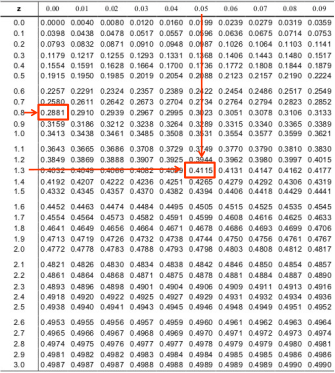
\includegraphics[scale=0.68]{img/z2.png}
\end{center}
\end{shaded}
\begin{shaded}
Regole di calcolo per normali standardizzati da tabelle per integrali:
\begin{itemize}
	\item integrali della forma $\int_{-\infty}^bf(u)\,du$:
	\begin{itemize}
		\item $b>0$, finito:
			\[\int_{-\infty}^b f(u)\, du= \frac{1}{2}+\int_0^b f(u)\, du\]
		\item $b<0$, finito:
			\[\int_{-\infty}^b f(u)\, du= \frac{1}{2}-\int_0^{-b} f(u)\, du\]
	\end{itemize}
	\item integrali della forma $\int_{a}^{+\infty}f(u)\,du$:
		\[\int_{a}^{+\infty}f(u)\,du= 1-\int_{-\infty}^{a} f(u)\, du\]
	\item integrali della forma $\int_{a}^{b}f(u)\,du$:
		\[\int_{a}^{b}f(u)\,du=\int_{-\infty}^bf(u)\,du-\int_{-\infty}^a f(u)\,du\]
\end{itemize}
\end{shaded}

Dopo aver considerato le distribuzioni principali continue, consideriamo 3 distribuzioni utili per la statistica inferenziale:
\begin{itemize}
    \item \textbf{chi-quadro}: siano $X_1, \cdots, X_n n$ variabili con distribuzione normale standard ed
        indipendenti tra loro e sia $X$ una variabile aleatoria definita come 
        \[ X = \sum X_i ^ 2 \]
        si dice distribuita secondo una chi-quadro con n gradi di liberta, indicata con $X \sim \chi_n^2$,
        che ovviamente essendo definita come somma di quadrati può assumere solo valori non negativi.

        \begin{figure}
            \caption{Distrubuzione chi-quadro}
	        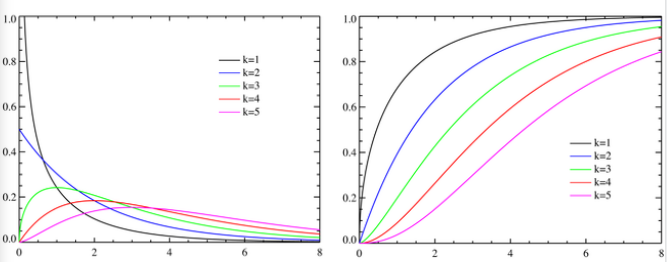
\includegraphics[scale=0.7]{img/chi.png}
        \end{figure}
    \item \textbf{t di student}: siano $Z \sim N(0, 1)$ e $Y \sim \chi_n^2$ due variabili indipendenti e
        sia $X$ una variabile aleatoria definita come 
        \[X = \frac{Z}{\sqrt{\frac{Y}{n}}}\]
        si dice distribuita secondo una t di student con n gradi di libertà, indicata con $X \sim t_n$.

        \begin{figure}
            \caption{Distribuzione t di student}
	        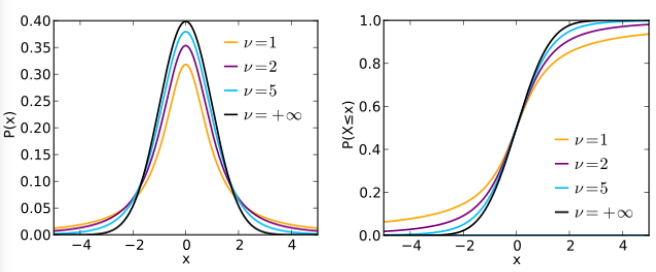
\includegraphics[scale=0.7]{img/t.png}
        \end{figure}

    \item \textbf{distrubuzione f}: siano $U \sim \chi_m^2$ e $V \sim \chi_n^2$ due variabili indipendenti, si
        ha che $X$ una variabile aleatoria definita come 
        \[X = \frac{\frac{U}{m}}{\frac{V}{n}}\]
        si dice distribuita secondo una $F$ con m e n gradi di libertà, indicata con $X \sim F(m, n)$.

        \begin{figure}
	        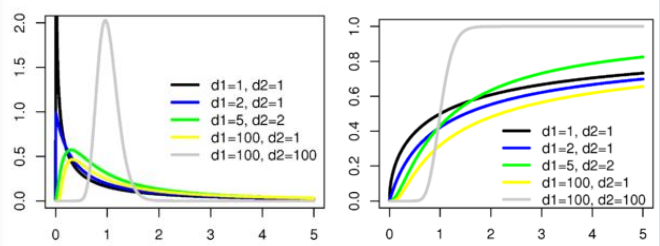
\includegraphics[scale=0.7]{img/f.png}
        \end{figure}
\end{itemize}

\chapter{Teoremi di Convergenza}
Consideriamo una successione $\{X_n, n \in \N\}$ di variabili aleatorie e sia $F_n$ la funzione di ripartizione
della generica variabile $X_n$ della successione.\newline
Diremo che la successione converge in distribuzione alla variabile $X$ avente funzione di ripartizione $F$ se vale:
\[\lim_{n\to\infty} F_n(t) = F(t)\]
per ogni $t \in \R$, punto di continuità per la funzione di ripartizione $F$. 

Si useranno le seguenti notazioni:
\[X_n\stackrel{d}{\longrightarrow} X\]
\[F_n\stackrel{d}{\longrightarrow} F\]
Nella definizione di convergenza in distribuzione vengono esclusi, nel passaggio al limite, i punti 
in cui la funzione di ripartizione limite $F$ è discontinua, per avere un concetto di convergenza simile all'intuizione.

Consideriamo ad esempio una successione di numeri reali $\{a_n, n \in \N\}$ tale che:
\[a_n \stackrel{d}{\longrightarrow} a \in \R \mbox{ per } n \to \infty\]
e pensiamo alle variabili aleatorie $X_n$ aventi funzione di ripartizione:
\[F_n(t) = \begin{cases}
            0 \mbox{ se } t < a_n\\
            1 \mbox{ se } t \geq a_n\\
           \end{cases}\]
ovvero la generica variabile $X_n$ assume valore $a_n$ con probabilità 1.\newline
Da un punto di vista intuitivo siamo portati a pensare che valga $X_n \stackrel{d}{\longrightarrow} X$,
con $X$ avente la funzione di ripartizione:
\[ F(t) = \begin{cases}
            0 \mbox{ se } t < a\\
            1 \mbox{ se } t \geq a\\
          \end{cases}\]
ovvero $X = a$ con probabilità uguale a uno ma la successione $\{a_n, n \in N\}$ tale che:
\[\begin{cases}
        a<a_n\mbox{ con n pari}\\
        a_n<a\mbox{ con n dispari}
  \end{cases}\]
risulta quindi:
\[\begin{cases}
    F_n(a) = 0 \mbox{ per n pari}\\
    F_n(a) = 1 \mbox{ per n dispari}
\end{cases}\]
il limite $\lim_{n \to \infty} F_n(a)$ non esiste quindi è scorretto dire che la successione converge
in distribuzione in quanto non è definibile in $a$ la funzione ripartizione limite $F$;
per evitare questi problemi si esclude, nella definizione di convergenza, i valori in cui la $F$ limite non è continua.

Segnaliamo che la convergenza in distribuzione non è l’unico tipo di convergenza tra variabili aleatorie
definito in letteratura, come ad esempio sono importanti convergenza quasi certa e in probabilità ma
in questo corso di statistica e probabilità abbiamo deciso di non considerarle, in quanto esula dagli scopi
e finalità del nostro corso.

\section{Legge dei Grandi Numeri}
Considero la successione $\{X_i \in \N_+\}$ di variabili aleatorie indipendenti ed identicamente distribuite e
considero poi la variabile aleatoria, detta \emph{media aritmetica n-esima della successione}
\[ \overline{X}_n = \frac{X_1 + \cdots + X_n}{n}\]

Avendo $E[X_i] = \mu$ e $V[X_i] = \sigma^2$, si ha allora $\overline{X}_n \stackrel{d}{\longrightarrow} M$,
con $M$ variabile aleatoria che assume il valore $\mu$ con probabilità 1.\newline
La proprietà appena introdotta costituisce una forma debole del risultato, noto con il nome di \emph{Legge dei Grandi Numeri}.

Nel dettaglio questa legge asserisce che:
\begin{teorema}
Se considero una successioni di variabili aleatorie indipendenti ed identicamente distribuite $\{X_i, i \in \N_+\}$
per cui esistono finiti valore atteso e varianza allora si può affermare che la successione:
\[\{\overline{X}_n, n \in \N_+\}\]
delle corrispondenti medie aritmetiche tende, al crescere di $n$, ad una variabile che assume certamente il valore:
\[E[X_i]=\mu\]
\end{teorema}
Quindi se considero una successione $\{x_i, i \in \N_+\}$ di realizzazioni delle variabili $\{X_i, i \in \N_+\}$
e considero la successione $\{\overline{x}, n \in \N_+\}$ delle corrispondenti realizzazioni delle medie aritmetiche,
abbiamo che questa seconda successione tende, per n tendente ad infinito, al valore $E[X_i] = \mu$.

Nella realtà le ipotesi della legge dei grandi numeri possono essere indebolite rispetto a quelle definite da
noi, infatti esistono versioni alternative in cui non è richiesta l'ipotesi che le variabili $X_i$ siano
identificamente distribuite.

La legge dei grandi numeri assicura la convergenza $\overline{X}_n \stackrel{d}{\longrightarrow} M$ ma non ci
fornisce alcuna informazione riguardo la rapidità con cui ciò avviene, infatti non sappiamo per quale $n$ è
lecito supporre che la realizzazione $\overline{x}_n$ assuma valore $\mu$ o prossimo ad esso.\newline
È intuitivo pensare che la convergenza avvenga con maggiore rapidità in caso di una varianza molto piccola, e
questo è il \emph{teorema del limite centrale}, in cui viene specificata quale sia la distribuzione della
variabile aleatoria $\overline{X}_n$, con $n$ sufficientemente grande, e quali siano il valore atteso e la
varianza della stessa.

Sia $\{X_i,\in\N_+\}$ una successione di variabili aleatorie che soddisfa le ipotesi della Legge dei Grandi
Numeri, ovvero siano le $X_i$ indipendenti ed identicamente Distribuite ed aventi valore atteso $\mu$ e 
varianza $\sigma^2$, entrambi esistenti e finiti.\newline
Si consideri ora la variabile aleatoria $S_n$, $S_n = \sum X_i$, in cui vale:
\[S_n \stackrel{d}{\longrightarrow} X \sim N(n \cdot \mu, \sqrt{n} \cdot \sigma) = N(n \cdot \mu, n \cdot \sigma^2)\].
Ovvero $S_n$ converge in distribuzione ad una variabile distribuita come una normale di media $n \cdot \mu$ e
deviazione standard $\sqrt{n} \cdot \sigma$.

Osservato che vale $\overline{X}_n = \frac{S_n}{n}$ dalla formula:
\[S_n \stackrel{d}{\longrightarrow} X \sim N(n \cdot \mu, \sqrt{n} \cdot \sigma) = N(n \cdot \mu, n \cdot \sigma^2)\]
si ha che $E[a \cdot X + b] = a \cdot E[X] + b,\,\, \forall X,\,\, \forall a,b \in \R$ e quindi:
\[E[\overline{X}_n] = E\left[\frac{S_n}{n}\right] = \frac{1}{n}E[S_n] = \frac{1}{n} E[X_1+\cdots +X_n] = \frac{1}{n}(n\mu) = \mu\]
inoltre si ha che $V[a \cdot X + b] = a^2 \cdot V[x],\,\, \forall X \,\, \forall a,b \in \R$ e quindi
\[V[\overline{X}_n]=V\left[\frac{S_n}{n}\right]=\frac{1}{n^2}V[S_n]=\frac{1}{n^2}V[X_1+\cdots+X_n]=\frac{1}{n^2}(n\sigma^2)=\frac{\sigma^2}{n}\]
quindi si conclude che:
\[S_n\stackrel{d}{\longrightarrow}X\sim N(\mu, \frac{\sigma}{\sqrt{n}})=N(\mu, \frac{\sigma^2}{n})\]
quindi per $n$ sufficientemente grande possiamo approssimare le variabili $S_n$ e $\overline{X}_n$ con delle variabili aventi distribuzione normale i cui parametri dipendono da quelli delle variabili $X_i$. Si ha inoltre la seguente approssimazione:\\
\textit{n è ritenuto sufficientemente grande sse $n\geq 30$}
\end{document}
